%
%                       This is a LaTeX 2e version of the
%                       laboratory project template file.
\documentclass[a4paper,12pt]{article}
\usepackage{fullpage, graphicx}
\usepackage[backend=biber, style=nature, sorting=none]{biblatex}
\addbibresource{shp_ref.bib}
\usepackage{subcaption}
\usepackage{listings}
\usepackage{color} %red, green, blue, yellow, cyan, magenta, black, white
\usepackage{siunitx}
\definecolor{mygreen}{rgb}{0,0.6,0}
\definecolor{mygray}{rgb}{0.5,0.5,0.5}
\definecolor{mymauve}{rgb}{0.58,0,0.82}

\lstset{ %
	backgroundcolor=\color{white},   % choose the background color
	basicstyle=\footnotesize,        % size of fonts used for the code
	breaklines=true,                 % automatic line breaking only at whitespace
	captionpos=b,                    % sets the caption-position to bottom
	commentstyle=\color{mygreen},    % comment style
	escapeinside={\%*}{*)},          % if you want to add LaTeX within your code
	keywordstyle=\color{blue},       % keyword style
	stringstyle=\color{mymauve},     % string literal style
}
%
%                       This section generates a title page
%                       Edit only the sections indicated to put
%                       in the project title, your name, supervisor,
%                       project length in weeks and submission date
%
\begin{document}
\pagestyle{empty}                       % No numbers of title page
\begin{minipage}[b]{110mm}
        {\Huge\bf School of Physics\\ and Astronomy
        \vspace*{17mm}}
\end{minipage}
\hfill
\begin{minipage}[t]{40mm}               
        \makebox[40mm]{
        
\includegraphics[width=4cm]{crest.pdf}}
\end{minipage}
\par\noindent                                           % Centre Title, and name
\vspace*{2cm}
\begin{center}
        \Large\bf \Large\bf Senior Honours Project\\
        \Large\bf Computational Physics\\[10pt]                     % Change to MP/CP/Astro
        \LARGE\bf Planetary Interiors: Studying The Phase Transition of Brucite        % Change to suit
\end{center}
\vspace*{0.3cm}
\begin{center}
        \bf Declan Mathews\\                           % Repace with your name
        \today                             % Submission Date
\end{center}
\vspace*{3mm}
%
%                       Insert your abstract HERE
%                       
\begin{abstract}
	%      The abstract is a short, concise explanation of the project
    %    covering the aims, outlines of techniques used and a short
    %    summary of the results. It should contain enough information to
    %    make the aims and success of the project clear, but contain no details.
    %    A typical abstract should be between 50 and 100 words.
       \noindent Using the Vienna Ab-initio Simultation Package (VASP), constant pressure structure optisimisations over 0-\SI{40}{\GPa} and then constant temperature molecular dynamics (MD) simulations over 300-1800\SI{}{\K} were ran on two phases, P$\bar{3}$m1 and P4$_3$2$_1$2, of Mg(OH)$_2$ (Brucite). A phase transition from P$\bar{3}$m1 to  P4$_3$2$_1$2 was expected to be found at roughly \SI{12}{\GPa}, based on the energy of the optimised states. This phase transition was found at between 10-\SI{20}{\GPa}. Superionic states of P$\bar3$m1 were expected at \SI{1200}{\K} and above for \SI{10}{\GPa} and above. These were found at 1500-\SI{1800}{\K} between 10-\SI{30}{\GPa} with diffusion constants of the order \SI{0.1}{\AA^2 \per\pico\second}. Further simulations would be required to fully define the phase boundary and study the properties more accurately.
        
\end{abstract}

\vspace*{0.5cm}

\subsubsection*{Declaration}

\begin{quotation}
\noindent I declare that this project and report is my own work.
\end{quotation}

\vspace*{1.5cm}
Signature: Declan Mathews\hspace*{7cm}Date: 29/11/2019

\vfill
{\bf Supervisor:} Dr. A. Hermann                % Change to suit
\hfill
10 Weeks                                         % Change to suit
\newpage
%
%                       End of Title Page
\tableofcontents                                % Makes Table of Contents
\newpage
\pagestyle{plain}                               % Page numbers at bottom
\setcounter{page}{1}                            % Set page number to 1
\section{Introduction}
%The introduction section of the report should introduce the project in
%more detail than in the abstract. In particular it should present the
%motivation, the aims, outline of techniques used, and the scope of the project. 
%It should also contain references to similar work in the
%same field to put your work in the correct context.
%As a general rule, people reading the abstract and introduction alone
%should have a good idea of the material in the project, the techniques
%employed and the results obtained. A typical introduction should be
%about 1 page, (300-450 words). 
Studying the Earth's interior experimentally can be incredibly difficult. However, these studies are key to understanding the processes and properites of materials in the interior and therfore those of the Earth as a whole, such as the geomagnetic field of the Earth and seismic activity. To study these, materials under extreme conditions can be modelled, simulated and the properties analysed from this data.

For this project, Brucite was studied under extreme conditions found in the Earth's mantle. Brucite has the formula Mg(OH)$_2$. The structure is trigonal in shape with space group symmetry P$\bar{3}$m1, shown in Figure \ref{Fig1}. The macroscopic shape is then formed from layers of this structure, in which each hydogen ion is below or above the middle of a triangle of three other hydrogen ions pointing towards it form the opposite layer \cite{HermannKey}. 
\begin{figure}[h!!!!]
	\centering
	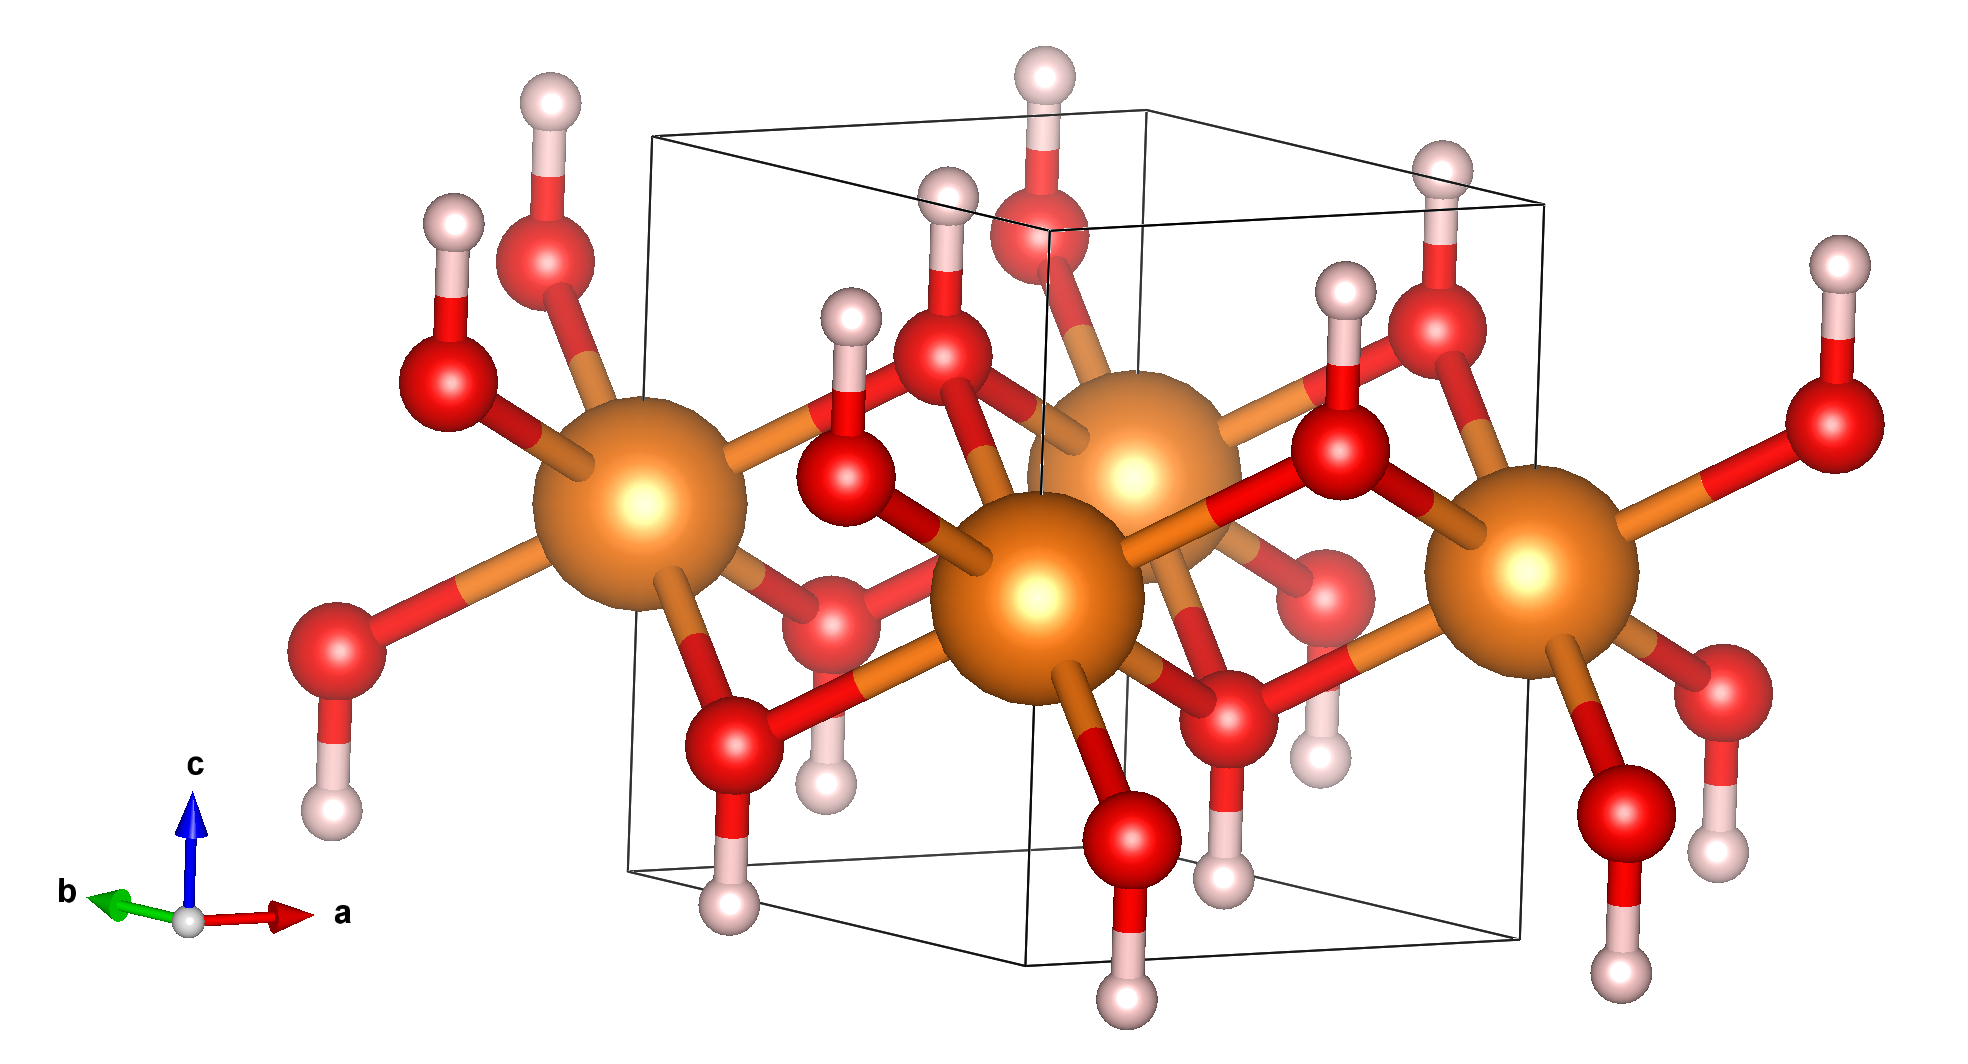
\includegraphics[width=10cm]{figures/p-3m1_p0_gs.png}
	\caption{Brucite P$\bar{3}$m1 phase at \SI{0}{\GPa}. Produced using VESTA \cite{VESTA}.}
	\label{Fig1}
\end{figure}

Brucite is a relatively simple hydrous molecule which is thought to be involved in the transportation of water in the Earth's mantle through the use of hydroxyl groups (OH) \cite{BELL1391, peacockwater}. The recent discovery of a higher pressure stable tetragonal phase (space group symmetry P4$_3$2$_1$2) suggests that it can be found much deeper in the mantle and is much more prevelant in the transportation than initially thought \cite{HermannKey}. Figure \ref{Fig2} shows the structure of the P4$_3$2$_1$2 unit cell. Through studying this phase transition, the transportation of water in the mantle can be better understood.
\begin{figure}[h!!!!]
	\centering
	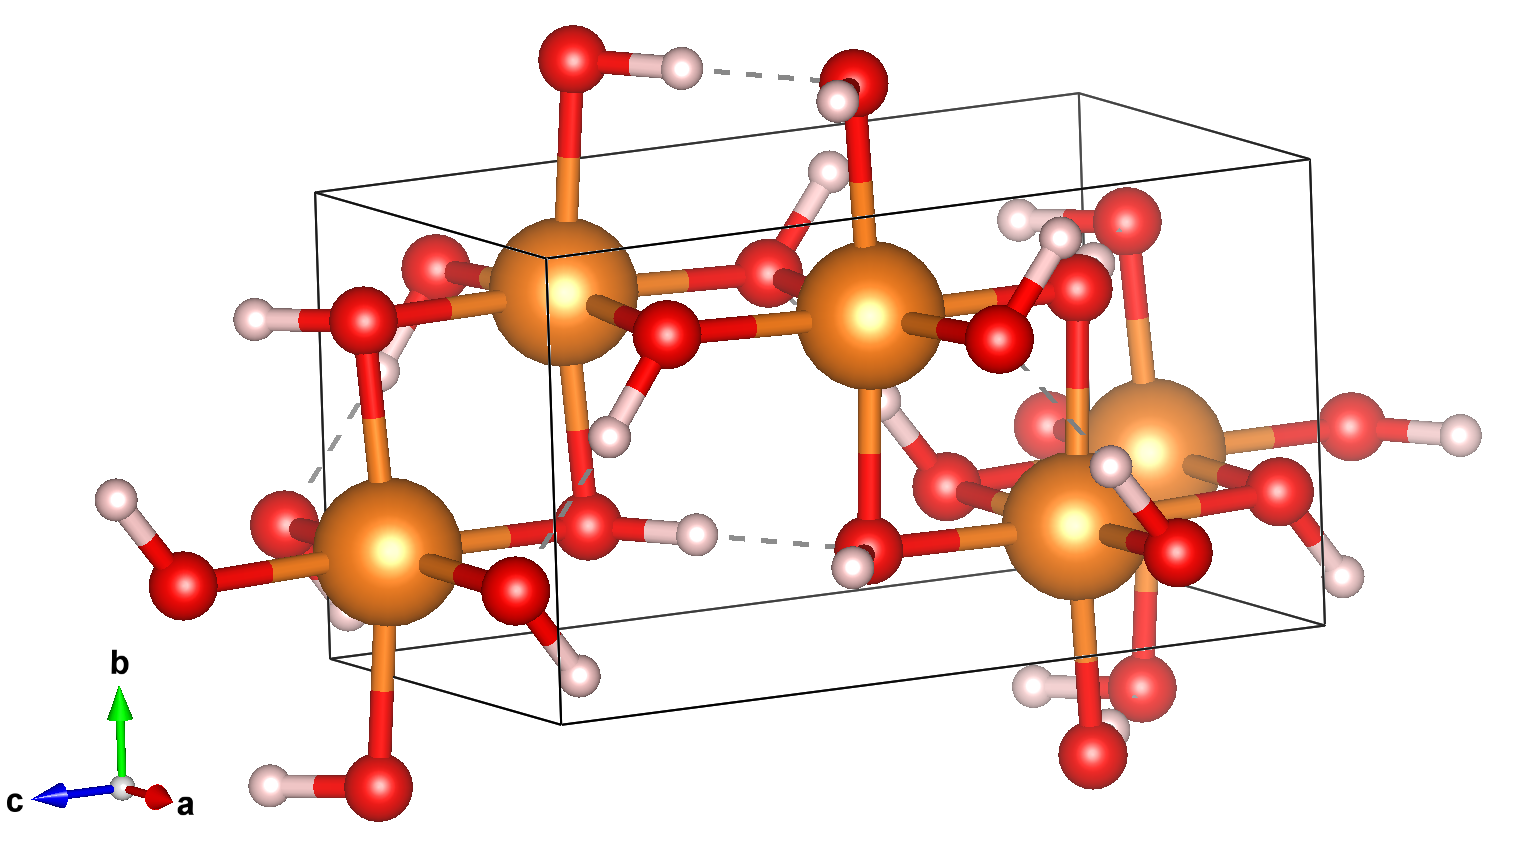
\includegraphics[width=10cm]{figures/p4_p0_gs.png}
	\caption{Brucite P4$_3$2$_1$2 phase at \SI{20}{\GPa}. Produced using VESTA.}
	\label{Fig2}
\end{figure}

Molecular dynamics (MD) simulations provide the data to study the phase transitions. First, optimised structures at varying pressures are found using the Vienna Ab-initio Simulation Package (VASP) \cite{VASP}. These optimised structures are then scaled up to form a super cell to be used in the MD. By scaling it up the assumption that the atoms are uncorrelated can be imposed and therefore the results treated as a macroscopic picture. If it had not been scaled up, the MD would only be ran on the unit cell atoms and the repeating units in the macroscopic picture would all follow the same correlated motion. MD simulations can then be ran using VASP as well. This is done using Density Functional Theory (DFT) on the computer Thomas at UCL \cite{THOMAS}. How DFT is employed will be dicussed further in the \textit{Background} section.

This project will study MD over 0-\SI{30}{\GPa} of pressure and 300-\SI{1800}{\K} for the P$\bar{3}$m1 phase and 20-\SI{40}{\GPa} and 300-\SI{1800}{\K} for the P4$_3$2$_1$2 phase. This is based on the suggestion of the supervisor and will be substantiated in the \textit{Methods} and \textit{Results and Discussions} sections. Using the collected data the mean square displacement (MSD), radial and partial distribution functions (RDF and PDF) can be produced. Using these in conjunction with the simulation viewing package, Visual Molecular Dynamics (VMD) \cite{VMD}, and mappings of the atom distributions, the states can be studied. From here, an estimation of the pressure-temperature (PT) graph can be produced.


\newpage
\section{Background}
%This section should cover the theory of the material in the project
%in sufficient detail to make the following work understandable to the
%average physicist. It should not contain large sections of standard
%bookwork, but should contain references to this material. The exact
%contents of this section will depend on the project being undertaken.
%This section should contain only the
%relevant theory. In particular a life history of the inventor of the
%technique to be used is
%totally irrelevant\footnote{I have seen a report that contained three pages
%on the life of Gabor, and it was not very interesting.}. Here use common sense
%and the general rule, ``If in doubt: leave it out'', however
%include information that you judge would be useful to one of your
%peers if they wehe to repeat the project. If you are
%undertaking a 12 week project and it includes a literature search, put the
%result of the search here. As a rough guide this section should be
%about 3-4 pages for a 6 week project, longer for longer projects.
%Note that if the project consists of a series of short experiments
%each of which requires a different theory and method, it may be appropriate
%to have one {\bf Theory, Method, Results} section for each
%experiment.

\subsection{Structure change}
The supercell structure of the P$\bar{3}$m1 phase is shown Figure \ref{Fig3}. From this it is clear to see each hydrogen will be surrounded by three other hydrogens facing towards it in a triangular shape. At low pressures these hydrogens are free to be above the oxygens, as the other hydrogens are far enough away for the Coulomb repulsion to be relatively small.
\begin{figure}[h!!!!]
	\centering
	\begin{subfigure}[t]{0.5\textwidth}
		\centering
		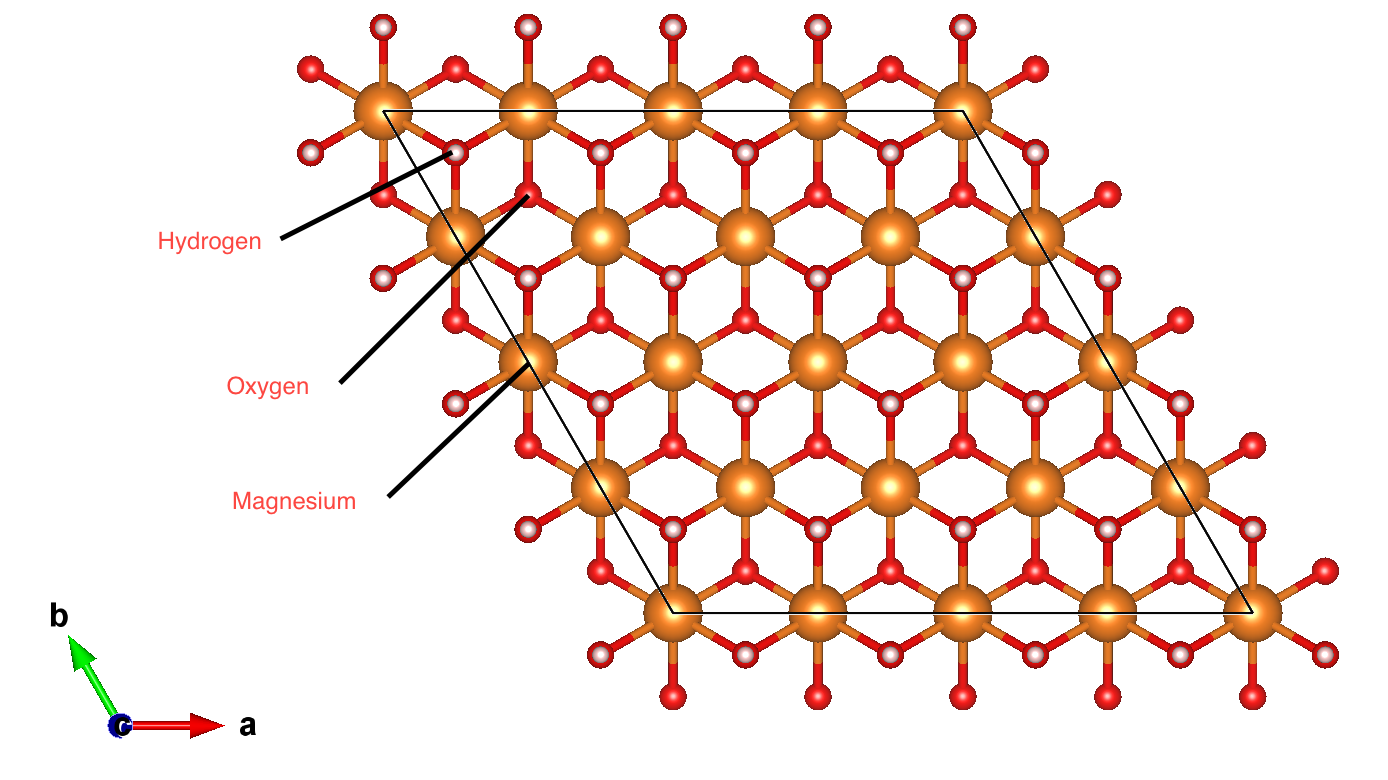
\includegraphics[width=7cm]{figures/p3m1_p0_supercell_top.png}
		\label{Fig3a}
	\end{subfigure}%
	\begin{subfigure}[t]{0.5\textwidth}
		\centering
		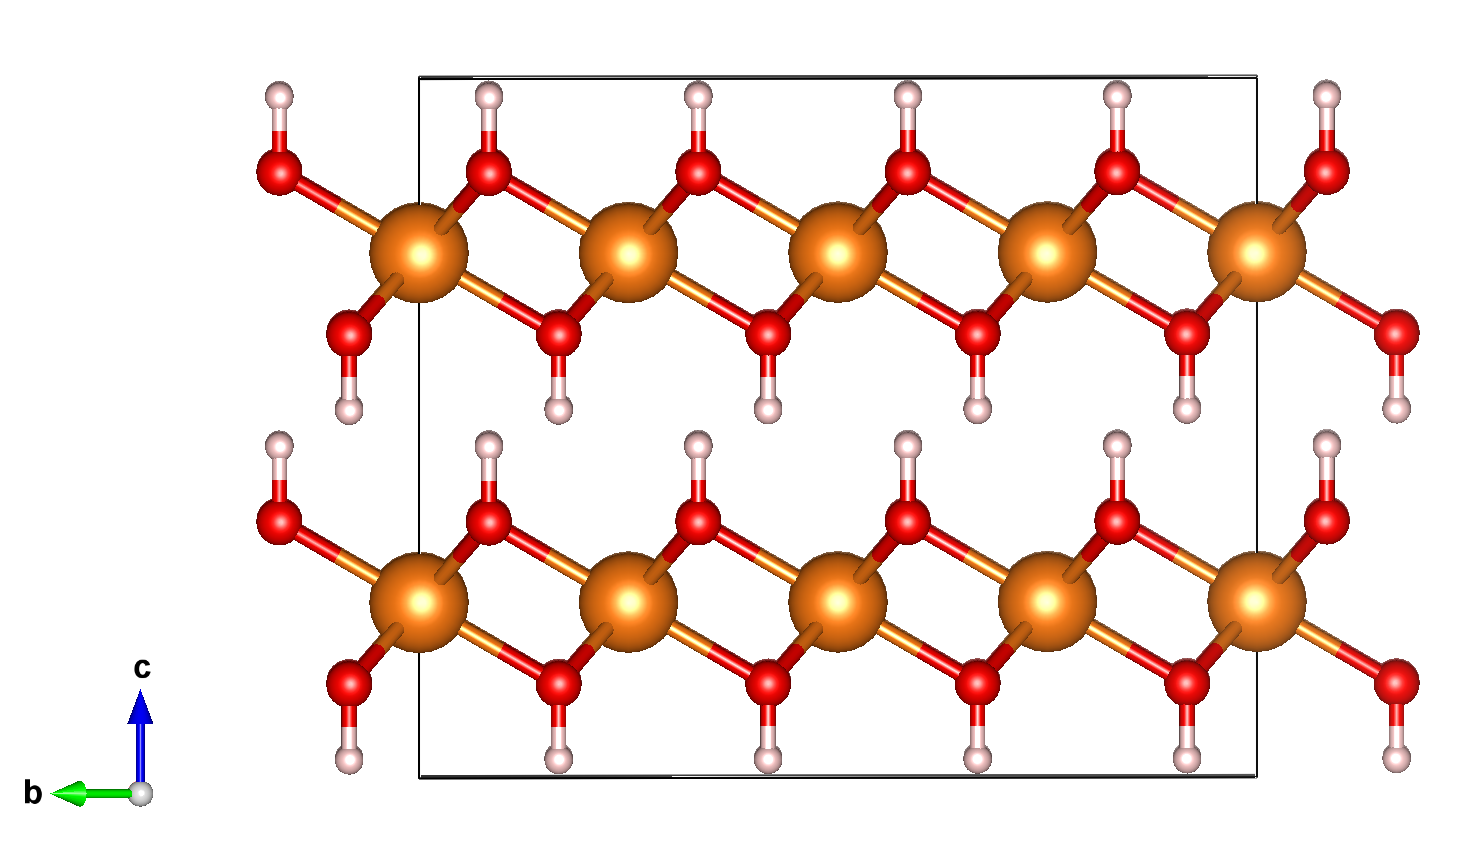
\includegraphics[width=7cm]{figures/p3m1_p0_supercell_front.png}
		\label{Fig3b}
	\end{subfigure}
	\caption{Brucite P$\bar{3}$m1 supercell at \SI{0}{\GPa} from above (left) and the front (right). Produced using VESTA.}
	\label{Fig3}
\end{figure}
However as the pressure is increased, the layers will get closer together and the hydrogens will no longer be able to remain directly above the oxygen. Each hydrogen will be repelled by the Coulomb force of the opposite hydrogens and attracted byt the opposite oxygens causing the bonds to become slanted. As these oxygen sites are already occupied by other hydrogens, frustration is caused \cite{RaugeiKey}. All the hydrogens will jump between the sites as an equilibirum state is trying to be achieved. This was documented by previous neutron diffraction studies \cite{PressHBond, Catti1995}. 

Once a certain pressure is reached it will become energetically favourable to be in the P4$_3$2$_1$2 phase, with supercell shown in Figure \ref{Fig4}. Here the OH groups form zigzagging chains amongst the tetragonal structure.
\begin{figure}[h!!!!]
	\centering
	\begin{subfigure}[t]{0.5\textwidth}
		\centering
		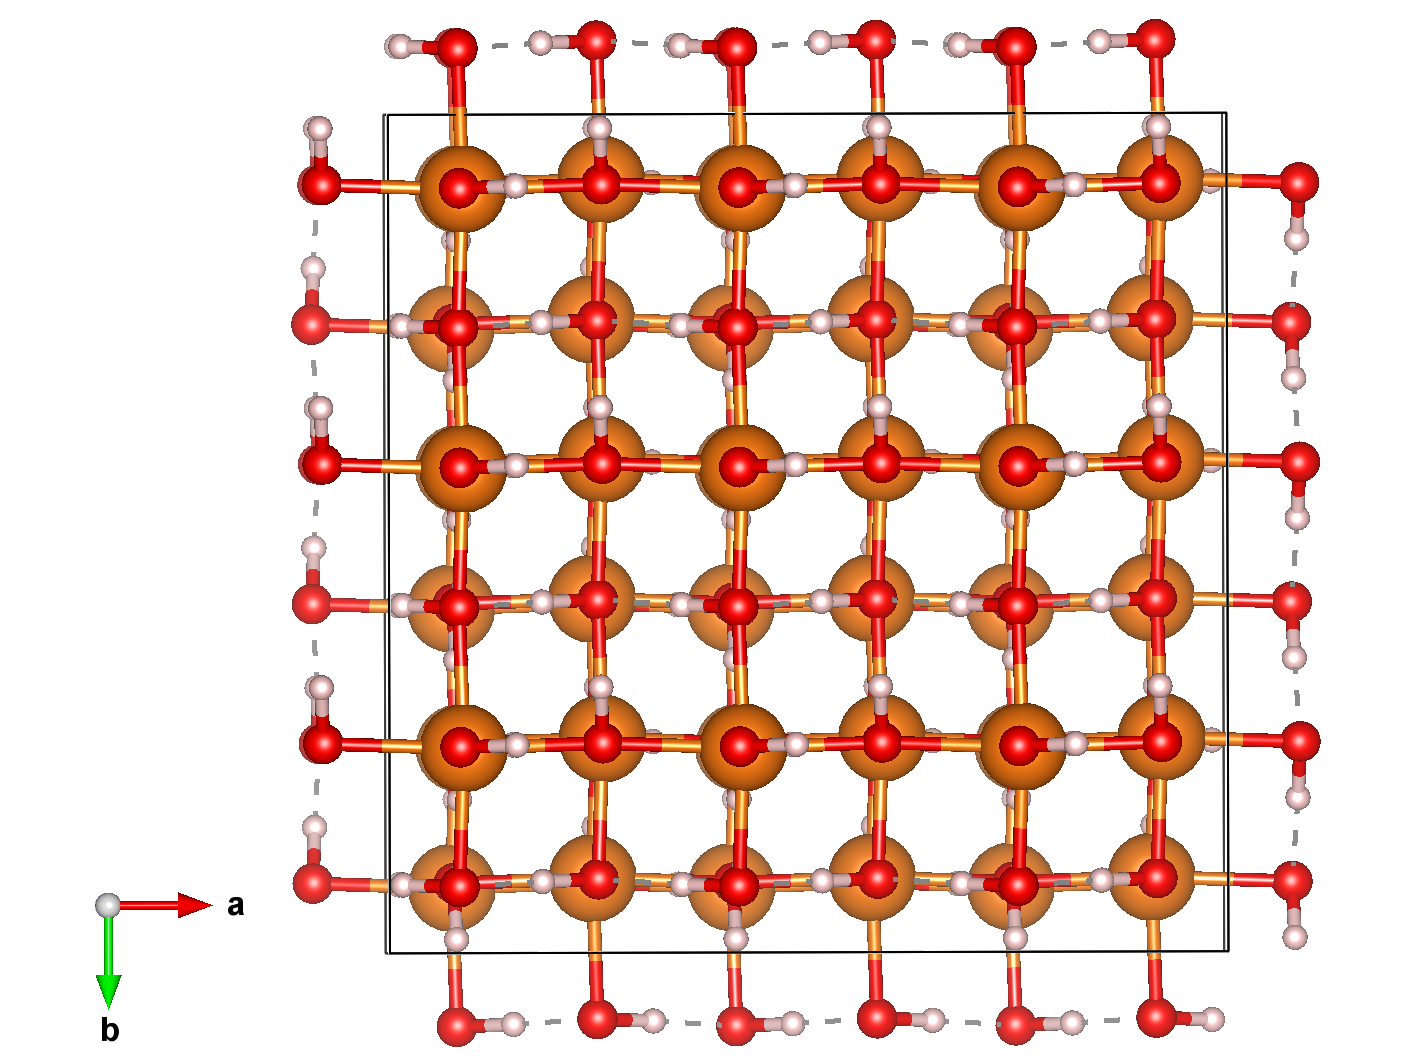
\includegraphics[width=7cm]{figures/p4_p200_supercell_above.png}
		\label{Fig4a}
	\end{subfigure}%
	\begin{subfigure}[t]{0.5\textwidth}
		\centering
		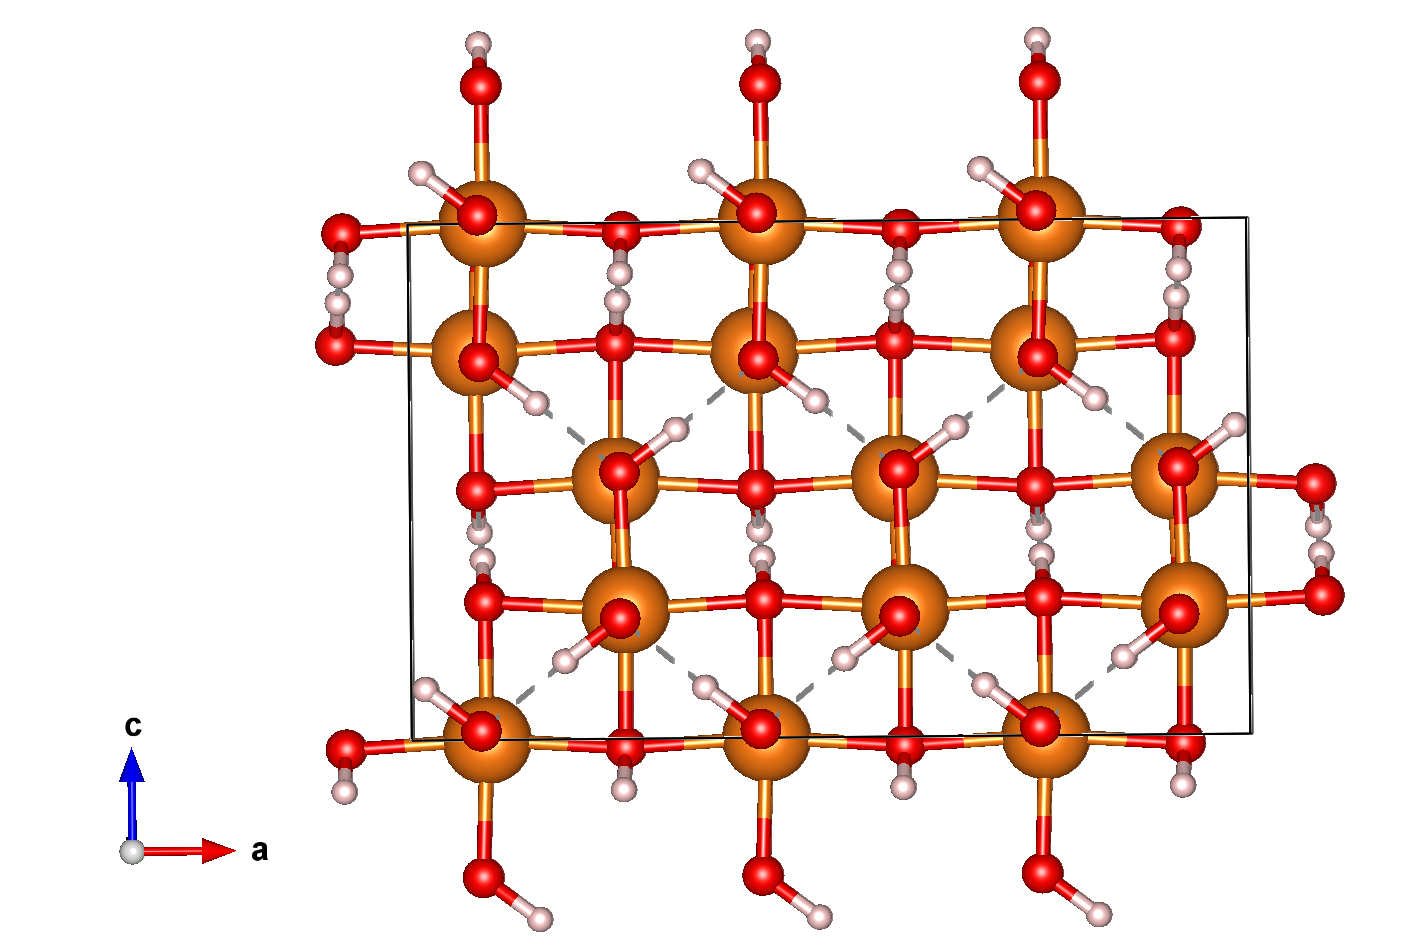
\includegraphics[width=7cm]{figures/p4_p200_supercell_side.png}
		\label{Fig4b}
	\end{subfigure}
	\caption{Brucite P4$_3$2$_1$2 supercell at \SI{20}{\GPa} from above (left) and the front (right). Produced using VESTA.}
	\label{Fig4}
\end{figure}

At higher temperatures, the ions will have more energy and so will vibrate and move about their positions more. This will increase the frustration in the P$\bar{3}$m1 phase and at high enough temperatures the hydorgen ions (protons) should become delocalised and form a 'sea' of free protons in between the layers, this is the superionic phase of P$\bar{3}$m1. As the protons aren't across individual layers in the the P4$_3$2$_1$2 it is not expected to form this same sea of protons. Beyond this state the decomposition of Brucite into magnesium oxide (MgO) and water (H$_2$O) is expected \cite{HermannKey}, but this will not be considered here.

\subsection{Molecular Dynamics (MD)}
Molecular dynamics is a large field with many different methods and techniques. Only a brief outline of denisty functional theory (DFT) and its implementation in this project will be discussed. For further information it would be best to seek textbooks and other papers directly discussing the topic, although several will be referenced to help explain key concepts.

\subsubsection{Density Functional Theory (DFT)}
%Many electron problem
%Cycle
%Kohn Sham Equation
%Exchange Correlation Functional
Density functional theory is a computational method based on solving the many body Schrödinger equation. Using the Born-Oppenheimer approximation \cite{BornOpp} the nuclei and electrons can be treated independently. The fixed positions of the nuclei can then be solved and the ground state energy of these written as a function of their positions. This is the \textit{adiabatic potential energy surface of the atoms}. The many electron Schrödinger equation then must be solved for the positions of the atoms to be defined.

This is where DFT is applied. The method is based on two fundamental principles layed out by Kohn and Hoenberg \cite{InhomegasHohenberg}. The two principles are \cite{DFTintro}:
\bigskip
\begin{enumerate}
 \item The ground state energy from Schrödinger's equation is a unique functional of the electron density.
 
 \item The electron density that minimizes the energy of the overall functional is the true electron density corresponding to the full solution of the Schrödinger equation.
\end{enumerate}
\bigskip
Using these principles the Kohn-Sham equations \cite{DFTintro, ExCKohnSham} were formulated, which have the form:

\bigskip
\begin{equation}
\left[ \frac{\hbar ^2}{2m} \nabla ^2 + V(\textbf{r}) + V_H (\textbf{r}) + V_{XC} (\textbf{r})  \right] \psi _i (\textbf{r}) = \epsilon _i \psi _i (\textbf{r})
\end{equation}
\bigskip

These equations are for single electron wavefunctions , where $\psi _i (\textbf{r})$ are the spatial components of the electron wavefunctions only. $V(\textbf{r})$ is the potential defining the electron ineteraction with the nuclei, $V_H (\textbf{r})$ is the Hartree potential and $V_{XC} (\textbf{r})$ is the exchange correlation potential. The Hartee potential describes the repulsive interaction between the electron and the electron gas (via a Coulomb potential), including an unphysical self interaction. The exchange correlation potential includes the correction to this self interaction and exchange and correlation terms. It is defined formally as a functional derivate of the exchange correlation energy \cite{DFTintro}:

\bigskip
\begin{equation}
V_{XC}(\textbf{r}) = \frac{\delta E_{XC}(\textbf{r})}{\delta n(\textbf{r})}
\end{equation}
\bigskip

Where $n(\textbf{r})$ is the electron density. The issue arising with these equations are that $n(\textbf{r})$ is required to define the Hartree potential, but to define $n(\textbf{r})$ the single electron wavefunctions must be know, which are found through solving the Kohn-Sham equations. To deal with this an iterative computational method is used \cite{DFTintro}:

\bigskip
\begin{enumerate}
\item Define an initial trial electron density $n(\textbf{r})$.

\item Solve Kohn-sham equations to find single electron wavefunctions $\psi _i (\textbf{r})$.

\item Calculate $n_{KS}(\textbf{r})$, the Kohn-Sham calculated electron density, from the calculated $\psi _i (\textbf{r})$.

\item Compare this $n_{KS}(\textbf{r})$ with the trial $n(\textbf{r})$, if they are equal, this is the ground state electron density. If they are not equal then an updated $n(\textbf{r})$ must be used and the process repeated.
\end{enumerate}
\bigskip

This is the overall process of DFT, with different methods of updating $n(\textbf{r})$ for different implementations. There is still one more key issue; $V(\textbf{r})$ and $V_H (\textbf{r})$ are known potentials, but $V_{XC} (\textbf{r})$ is not. The only case in which this functional is known exactly is for a uniform electron gas \cite{Constantin, PerdewJohnWang}. However, there has been much research into developing accurate exchange correlation functionals\footnote{There has actually been a study into how we are straying further from an ideal functional \cite{Medvedev49}, likely due to the development of specific functionals fit for certain purposes.}. For more information on other functionals see \cite{DFTintro, DFTA}.

For this project a particular \textit{Generalised Gradient Approximation (GGA)} functional was used, this being the \textit{Perdew-Burke-Ernzerhof (PBE)} functional \cite{AssessPBE, PBE}. This uses information on the local electron density and the local gradient of the electron density, however, a full description is beyond the scope of this project.
\bigskip

\noindent Finally, in order to solve the Kohn-Sham equations and find a self-consistent solution, the electron wavefunctions must be expanded in a basis set. In VASP, this is done using a plane wave basis set, as it is much more computationally efficient for MD \cite{PAWintro}. These are of the form:

\begin{equation}
u_n (\textbf{r}) \propto e^{i (\textbf{G} \cdot \textbf{r})}
\end{equation}

Where $\textbf{G}$ is the reciprocal lattice vector. To truncate these an energy cutoff value is introduced \cite{VASP}, which sets all coefficients of planewaves with values above this to zero.

\begin{equation}
|\textbf{G} + \textbf{k}| < G_{cut} \quad \mathrm{and} \quad E_{cut} = \frac{\hbar ^2}{2m}G_{cut}
\end{equation}
\bigskip

This means that the plane wave expansion does not completely converge, but the complete convergence is usually unnecessary and the computational expense saved can be significant.

\subsection{Vienna Ab-initio Simulation Package (VASP)}

This section will provide an overview of VASP to provide a working knowledge of its use in the project. Further information can be found in its documentation \cite{VASP}.

\subsubsection{Input files}

Simulations are ran based on four main input files, named \textit{INCAR}, \textit{POSCAR}, \textit{POTCAR} and \textit{KPOINTS}.
\begin{itemize}
\item \textit{POSCAR} describes the atoms/ions in the cell, their positions and the overall structure.

\item \textit{KPOINTS} states the number and location of the $k$-points, or allows the package to automatically determine them.

\item \textit{INCAR} is the main input file for settings to determine the type and method of simulation ran. The settings for the simulations used in this project will be included in the appendix.

\item Finally, \textit{POTCAR} details the pseudo-potentials for the cell used in the simulation for the \textit{projector augmented wave method (PAW)}. The principle behind these is to reduce computational cost by approximating the potentials used in the calculation as part of the plane wave basis set expansion. The specifics are not necessary for the understanding of this project but more can be found at \cite{DFTintro, DFTA, PAWintro}.
\end{itemize}

\subsubsection{$k$-point sampling}

By Bloch's theorem \cite{Bloch1929} we know that for a periodic crystal we only need to consider the first Brillouin zone to describe the crystal. To efficiently compute the solutions, $k$-point sampling is used by selecting appropriate points in reciprocal space to approximate the solution (see Figure \ref{Fig5} for visualisation). The more $k$-points selected the higher the accuracy of the approximation. However, the computational cost increases vary rapidly with number of $k$-points.

\begin{figure}[h!!!!]
	\centering
	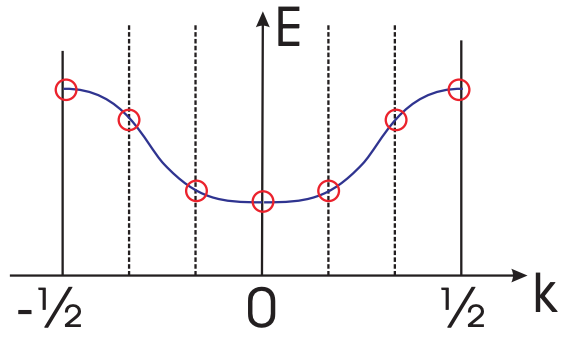
\includegraphics[width=10cm]{figures/kpointsamp.png}
	\caption{$k$-point sampling visualisation. Image sourced from \cite{KPoints}}
	\label{Fig5}
\end{figure}

For the ground state optimisations, the $k$-points selection was done automicatically by VASP, further details will be provided in \textit{Methods} and \textit{Results and Discussion}. As there were multiple $k$-points chosen by VASP, the parellisation of Thomas was taken used. This is represented by the \textit{KPAR} setting in the \textit{INCAR} file.

To save on computational cost only one $k$-point was selected for the MD at the advice of the supervisor. This was based on the Baldereschi point \cite{Baldereschi} and here was used as [0.25, 0.25, 0.25] ([0, 0, 0] and [1, 1, 1] being the far corners of the supercell) in units of the supercell basis vectors. As there was only one $k$-point, no parellisation was used so there is no \textit{KPAR} setting in the \textit{INCAR} file.

\subsubsection{Structure optimisation at constant pressure}

Structure optimisation is done through minimising the energy of the structure by varying the shape and size of the cell and positions of the atoms inside it. The external pressure is defined in the input and an iterative process to calculate the optimum structure is carried out. 

\subsubsection{MD}

The selected methods in VASP for the MD DFT calculations were PAW PBE, as discussed above. These were used to calculate the the positions of the atoms after each time step in the NVE ensemble, also known as the microcononical ensemble \cite{GTherm}.

The temperature was chosen for each run and the calculations for each step were based on the equation of state for constant number of constituent particles, volume and total energy. A temperature beginning and end is defined for this ensemble and by setting these to the same value 'constant' temperature simultations can be ran. The temperature will actually flucuate about this value (and will do so in a manner determined by the \textit{SMASS} setting, discussed in the \textit{Methods} section).

Having already optimised the structure at constant pressure for the simulation, the result is effectively what the MD would look like at this particular pressure and temperature(the pressure is actually above the optimising pressure, but to save on volume of data output the actual pressure was not written out, this will reviewed further in the \textit{Results and Discussion} section).

\subsection{Analysis techniques}

This section provides an overview of the main techniques and a general idea of what they represent.

\subsubsection{Mean Square Displacement (MSD)}

The mean square displacement (MSD) is a measure of how far something has moved from its original position after a set time. The equation defining it is \cite{Compmod}:

\smallskip
\begin{equation}
MSD(t) = \langle |\textbf{r}(t) - \textbf{r}_0 |^2 \rangle = \frac{1}{N} \sum_{i}^{} |\textbf{r}_i(t) - \textbf{r}_{i0} |^2
\end{equation}
\smallskip

For a particle moving away from its original position the MSD will have a positive gradient, and the particle is diffuse. If there is no gradient the particle is staying at its original position and is bound (although it will more than likely have flucuations about this point). This applies to multiple particles as well.

\begin{figure}[h!!!!!!!!!!!!!!!!!!!!!!!!!!]
	\centering
	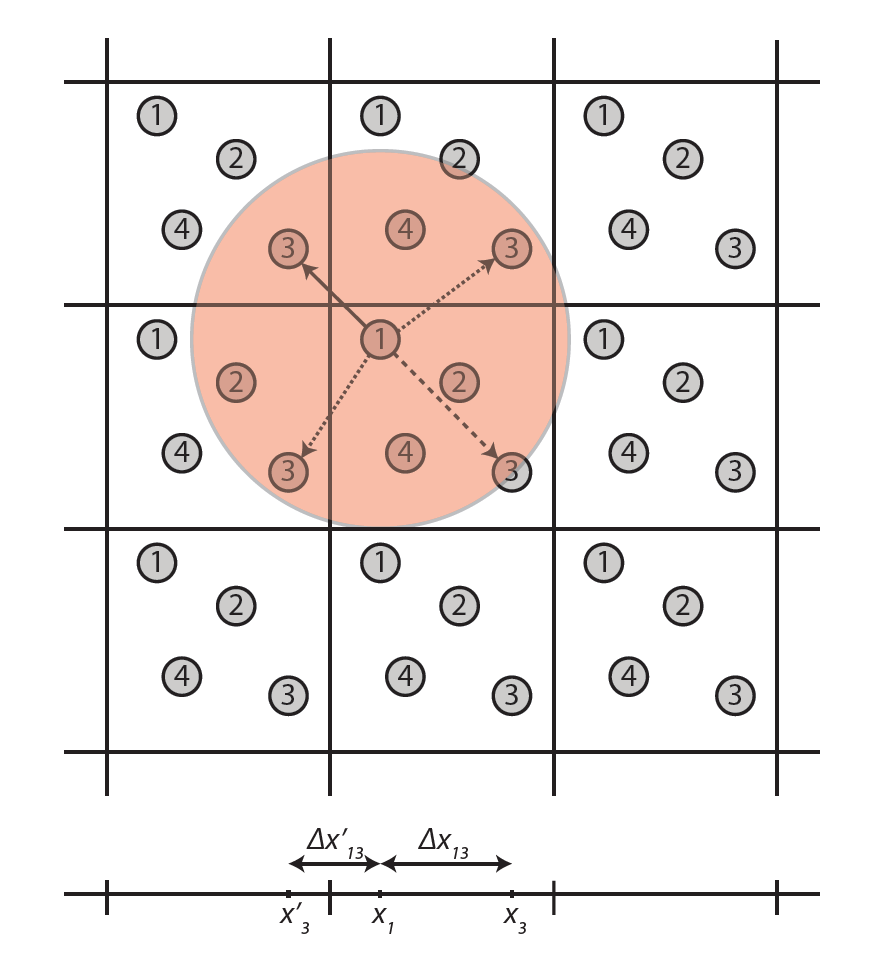
\includegraphics[width=7.5cm]{figures/minimag.png}
	\caption{A simple 2D orthogonal example of the minimum image convention. The dotted lines are distances to possible images, the solid line is the closest image and the correct distance to use. Image sourced from \cite{Compmod}}
	\label{Fig6}
\end{figure}

A key principle that must be adhered to for periodic systems, such as this one, is the \textbf{minimum image convention} \cite{Compmod}. This requires that the closest particle distance be used and as the system is periodic it could be in the 'image' of the cell in any direction, as shown in Figure \ref{Fig6}. 

From the MSD the diffusion constant can also be found using the following equation:

\begin{equation}
MSD(t) = 2dDt
\end{equation}

Where d is the number of dimensions, t is the time and D is the diffusion constant. For the P$\bar3$m1 phase, the number of dimensions chosen is two, as the hydrogens move around in the planes (they do move slightly in the third dimension but this is negligible). This can be found by finding the gradient of the increasing section of the MSD before the plateau.

\subsubsection{Radial Distribution Function (RDF) and Partial Distribution Function (PDF)}

The RDF represents the distribution of ions in the cell and shows a measure of the probability of finding the atom at a particular point. This can show the ordering of the system, and can be applied to only certain atoms or atom pairs, which generates a PDF. The RDF and PDF also need to abide by the minimum image convention. It is represented by the equation \cite{Compmod}:

\begin{equation}
RDF(r) = \frac{1}{N_\rho} \langle \sum_{i,j}^{} \delta (r_{ij} - r) \rangle
\end{equation}

Where $i,j$ are the ion pairs. $N_\rho$ is the normalisation factor and is determined by \cite{Compmod}:

\medskip
\begin{equation}
N_\rho = 4\pi \rho r^2 dr
\end{equation}
\medskip

Here, $\rho$ is the density of ion pairs and r is the distance between the ions.


\newpage
\section{Method}
%This section should contain the details of the method employed. 
%As in the previous sections standard techniques should not be written
%out in detail. For example if you use an oscilloscope to take a
%measurement, the theory of the CRO tube\footnote{Don't laugh, I have actually
%seen this.} is {\bf not relevant}. In computational projects this
%section should be used to explain the algorithms used and the layout of
%the computational code. Long detailed sections of theory, data tables
%and details of computational code used in data analysis only should not
%appear in this section, but should/may be included in the appendices.
%
%This section should emphasise the philosophy of the approach used
%and detail novel techniques. However
%please note: this section is {\bf not} a blow-by-blow account of what
%you did throughout the project, and in particular it should {\bf not} 
%contain large detailed sections about things you tried and found to be
%completely wrong. Remember you are writing a technical report, and
%not a diary. If however you find that a technique that was expected to
%work failed, that is a valid result and should be included.
%
%Here logical structure is particularly important, and you may find that
%to maintain good structure you may have to present the experiments
%in a different order from the one in which you carried them out.
%

\subsection{Structure optimisation and energy of ground state phases comparison}
Using VASP, the optimised structures of both P$\bar{3}$m1 and P4$_3$2$_1$2 unit cells were found at \SI{5}{\GPa} intervals between 0-\SI{40}{\GPa} (0 being found at \SI{1}{\bar} = \SI{0.01}{\GPa}; essentially zero pressure). A plane wave energy cut off (\textit{ENCUT}) was chosen as \SI{400}{\eV} as per the supervisors suggestion. The energy convergence threshold (\textit{EDIFF}) was initially chosen as \SI{1e-5}{\eV \AA ^{-1}} but the simulations were failing as it was too high, so a lower value of \SI{1e-7}{\eV \AA ^{-1}} was chosen. They were optimised three times, using the final point of the last optimisation as a starting point for the next, at each pressure for each phase. The energy of these was written out to a file and a python programme was written to read in the data and plot the energy difference between the phases over the pressure range.

\subsection{MD pressure and temperature values}
Using this and the supervisors suggestion, the pressure and temperature values for each phase for the MD simulations were chosen. For the P$\bar{3}$m1 phase, MD was ran for the optimised states at \SI{0}{\GPa} (effectively), \SI{5}{\GPa}, \SI{10}{\GPa}, \SI{20}{\GPa} and \SI{30}{\GPa}. For each pressure value the simulation was carried out at \SI{300}{\K}, \SI{600}{\K}, \SI{900}{\K}, \SI{1200}{\K}, \SI{1500}{\K} and \SI{1800}{\K}. For the P4$_3$2$_1$2 phase, the pressure values were \SI{20}{\GPa}, \SI{30}{\GPa} and \SI{40}{\GPa}. The temperature values were the same as the P$\bar{3}$m1 phase. 

\subsection{MD settings}
All MD was ran with the energy cutoff value of \SI{400}{\eV} and an energy convergence threshold of \SI{1e-6}{\eV \AA ^{-1}}. This was increased from \SI{1e-7}{\eV \AA ^{-1}} to reduce the computational cost at no significant accuracy decrease. A supercell size of $4\times 4 \times 2$ of the unit cell for P$\bar{3}$m1 and $3 \times 3 \times 1$ for P4$_3$2$_1$2 was chosen. These offered roughly the same number of ions in total (160 and 180 respectively) and allowed for the results to be considered a macroscopic crystal view as there was less correlation on the movement of particles when the crystal is scaled up macrospocially through the periodicity of the crystal.

\subsection{SMASS testing and setting}
A test on the effect of the \textit{SMASS} setting was carried out before the MD data was gathered. Three seperate simulations were ran at \SI{0}{\GPa} and \SI{600}{\K} on the P$\bar{3}$m1 phase with \textit{SMASS} $=1, 3 \, \mathrm{and} \, 10$. This was done to get an approriate frequency and amplitude of the temperature flucuation ensuring it was as sufficiently close to 'constant' temperature but not creating an unphysical situation through artificially pushing the system towards 'constant' temperature. The \textit{SMASS} value chosen in the end was 1 and is stated here as it is a setting used in all MD results.

\subsection{MSD}
A python programme was written to calculate the MSD at a sampling rate determined by the user. This programme used class structure storing the input data as 'self' to allow reuse as necessary. It output the results to three seperate files for the magnesium, oxygen and hydrogen MSD data to allow different programmes to be written to analyse the data  by varying methods without having to regather all the data.

The data was read in from the \texttt{.xml} files produced using ElementTree \cite{ETree}. This being the initial positions, all subsequent positions at each step and the matrix of the basis set used to describe the supercell by VASP (named in the programme as \texttt{L}).

The diffusivity was found by selecting the increasing sections of the superionic data, plotting the data, finding the linear line of best fit and its gradient and using the equation mentioned in the \textit{Background} to calculate the diffusivity.

\subsubsection{Dealing with minimum image convention}
The main issue was dealing with the minimum image convention, as the cell was non orthogonal the cell horizontally in the $ab$ plane (as seen in Figure \ref{Fig3}). However, as the $c$ plane is orthogonal to the others, this was tackled by seperating the positions into two seperate lists for $ab$ and $c$ components and using different methods for each. The $c$ components could be delt with simply by using the below class method:

\smallskip
\lstinputlisting[firstline=180, lastline=189, language=Python]{Files/MSDP.py}
\smallskip

The $ab$ components were trickier to deal with and a brute force method was used. The code is longer and so will instead be included in the appendix. However,the idea is relatively simple. This involved creating a list of the image positions in the plane surrounding (as seen orthogonally in Figure \ref{Fig6}), finding the Euclidian distance between the ions in question and updating the minimum distance to be returned if a new minimum is found.
\bigskip

\noindent Using Pythagoras' theorem, the shortest Euclidian distance between the ion at the current timestep and its initial position was found. This was returned to another method which was used to iterate over all the ions of each type as required to then total, normalise and append the MSD to individual lists for each ion type. This method made use of a \texttt{check} value which controlled the sampling rate. When all the samples were taken, the three individual lists were appended to a final 2D list which was returned and written out to individual files. Seperate programmes were written to graph the data.

\subsection{RDFs and PDFs}

The RDF and PDF used many of the same methods as the MSD, mainly the few described above for dealing with the minimum image convention. The differences being that it wasn't atoms being compared to their initial positions, but to other atoms at the same time step. This also changed the iterative method to calculate the RDF and PDF.

The largest difference was the normalisation of the RDF and PDF. The method to do this normalisation was:

\smallskip
\lstinputlisting[firstline=188, lastline=197, language=Python]{Files/RDF.py}
\smallskip

Where \texttt{numatoms} was the number of atoms in consideration, \texttt{numruns} was the total number of runs sampled, \texttt{dr} was the bin size and \texttt{rdf} was the unnormalised RDF (or PDF).

\subsection{Simulation viewing, structure production and distribution mapping}

The entire simulation could be viewed using Visualis Molecular Dynamics (VMD), which also allowed some images of the distributions of atoms throughout the simulation to be produced. This was used to follow up on features seen in the MSD and RDF/PDF and to visualise what the simulation looks like.

Visualisation for Electronic and STructural Analysis (VESTA) was used produce images of the cells that could be rotated and studied and to created the supercells from the unit cells to be used in the simulations.

The supervisor provided a python programme which mapped the hydrogen ion distributions of the simulations back onto the unit cell. This was studied in VESTA, with the hydrogen distributions shown as isosurfaces (coloured 3D shapes) to view their overall movement.


\newpage
\section{Results \& Discussion}
%
%This section should detail the obtained results in a clear,
%easy-to-follow manner. Remember long tables of numbers are just as boring to
%read as they are to type-in. Use graphs to present your results where
%-ever practicable. When quoting results or measurements
%{\bf DO NOT FORGET ABOUT ERRORS}. Remember there are two basic types
%of errors, these being random and systematic, which you must consider.
%Remember also the difference between an error and a mistake, computer
%program bugs are mistakes.
% 
%Again be selective in what you include. Half a dozen
%tables that contain totally wrong data you collected while you forgot
%to switch on the power supply are {\bf not relevant} and will frequently
%mask the correct results. 
%
%This section must contain a discussion of the results. This should
%include a discussion of the experimental and/or numerical errors, and a
%comparison with the predictions of the background and theory underlying
%the techniques used. This section should highlight particular strengths
%and/or weaknesses of the methods used.

\subsection{Structure optimisation energies}

Once the structures had been optimised, the difference in energy of the two phases was plotted for each pressure and is shown in Figure 7.

\begin{figure}[h!!!!!]
	\centering
	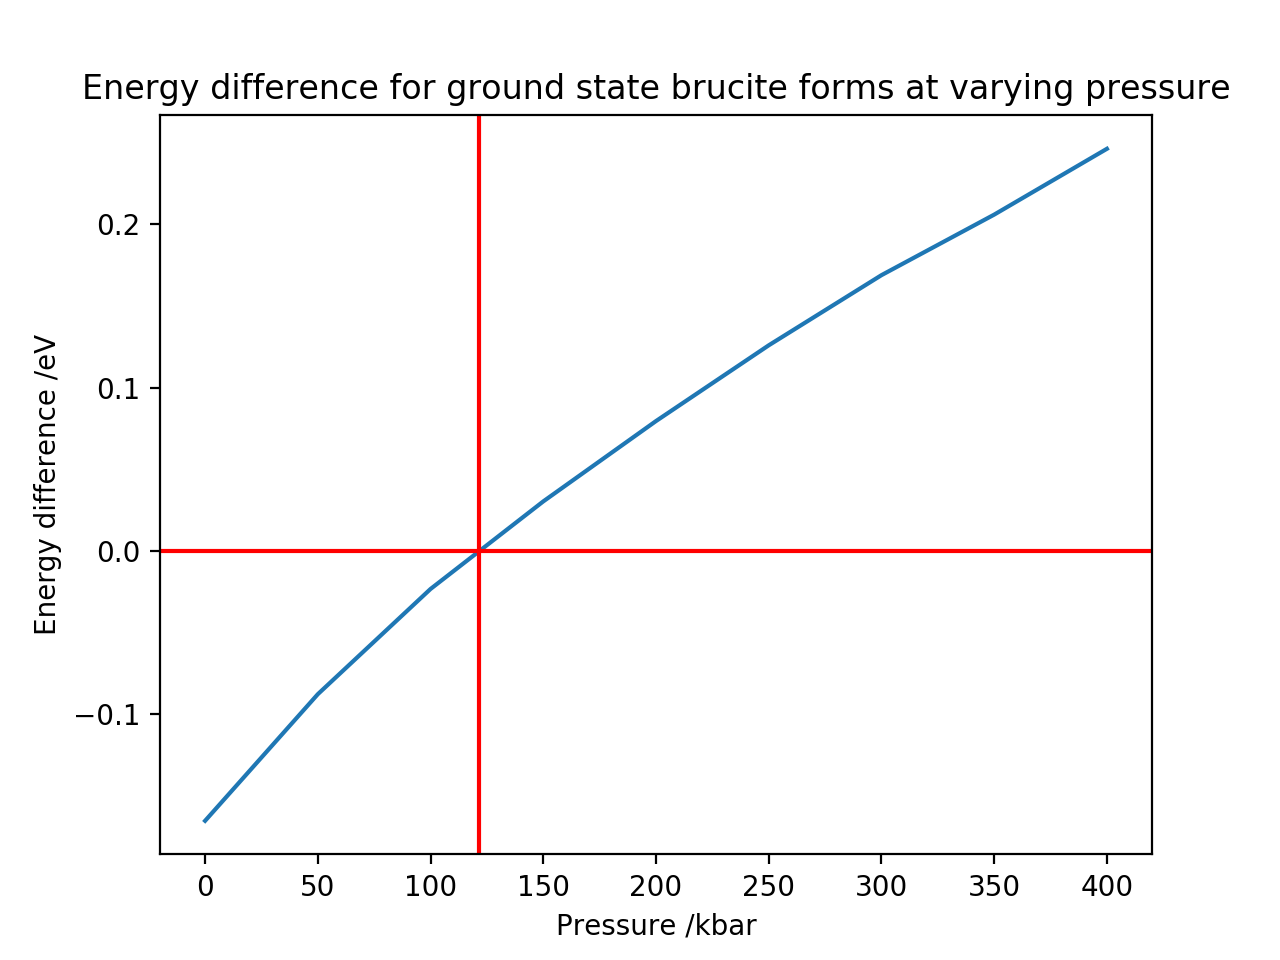
\includegraphics[width=8cm]{figures/ediff_GS_pvary_ex.png}
	\caption{The energy difference of the optimised structures of P$\bar3$m1 minus P4$_3$2$_1$2 at varying pressure. The red lines show the point when the energy difference becomes positive.}
	\label{Fig7}
\end{figure}

In Figure \ref{Fig7} the red lines show when the energy difference (of P$\bar3$m1 minus P4$_3$2$_1$2) becomes positive. This means the energy for P4$_3$2$_1$2 is lower past this point and so it is expected to be a more favourable state. We can see this happens at roughly \SI{120}{\kilo\bar} (\SI{12}{\GPa}) however there are only nine data points on this graph and so it is only a very rough estimate. From this it can be hypothesised that above \SI{12}{\GPa} brucite should adopt the P4$_3$2$_1$2 structure. Using this graph the pressures for the MD simulations of each structure were decided so that the possible phase transition could be studied. The optimised unit cell structures used in the \textit{POSCAR} files for beginning the MD are included in the appendix for reference.

\subsection{MSD}

The results for the MSD of the hydrogen ions for the P$\bar{3}$m1 phase are presented in Figure \ref{Fig7} and the results for P4$_3$2$_1$2 phase are shown in Figure \ref{Fig8}.

\begin{figure}[h!!!!!!!!!!!!!!!!!!!!!]
	\centering
	\begin{subfigure}[t]{0.5\textwidth}
		\centering
		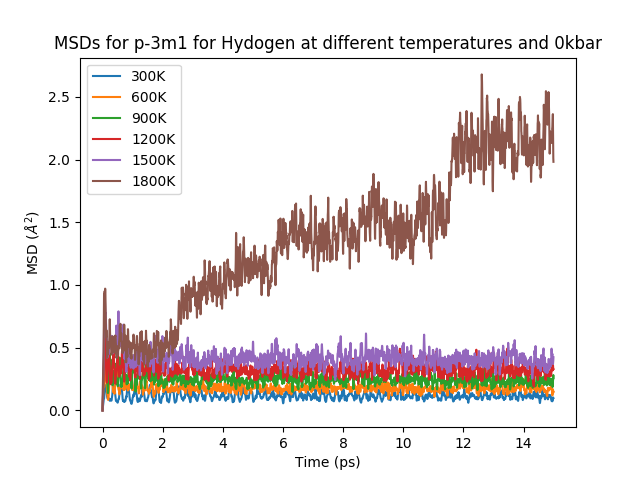
\includegraphics[width=7cm]{figures/p3m1_msd_H_p0.png}
		\subcaption{P$\bar{3}$m1 \SI{0}{\GPa}}		
		\label{Fig8a}
	\end{subfigure}%
	\begin{subfigure}[t]{0.5\textwidth}
		\centering
		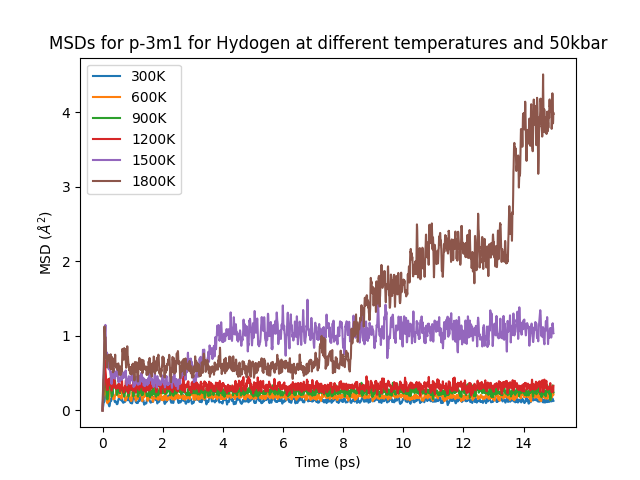
\includegraphics[width=7cm]{figures/p3m1_msd_H_p50.png}
		\subcaption{P$\bar{3}$m1 \SI{5}{\GPa}}
		\label{Fig8b}
	\end{subfigure}%
\\
	\begin{subfigure}[t]{0.5\textwidth}
	\centering
	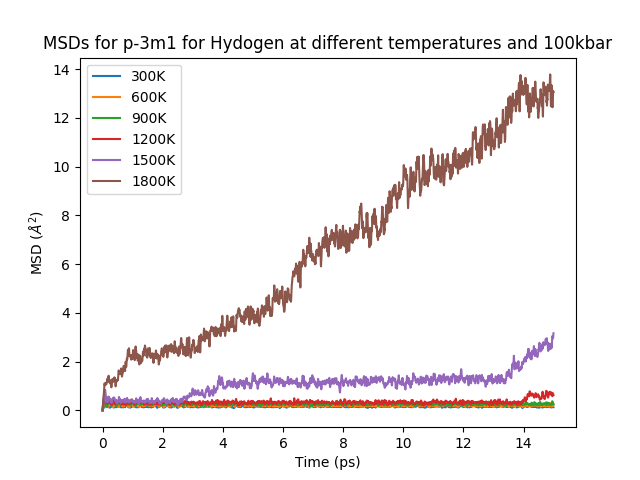
\includegraphics[width=7cm]{figures/p3m1_msd_H_p100.png}
	\subcaption{P$\bar{3}$m1 \SI{10}{\GPa}}
	\label{Fig8c}
\end{subfigure}%
	\begin{subfigure}[t]{0.5\textwidth}
	\centering
	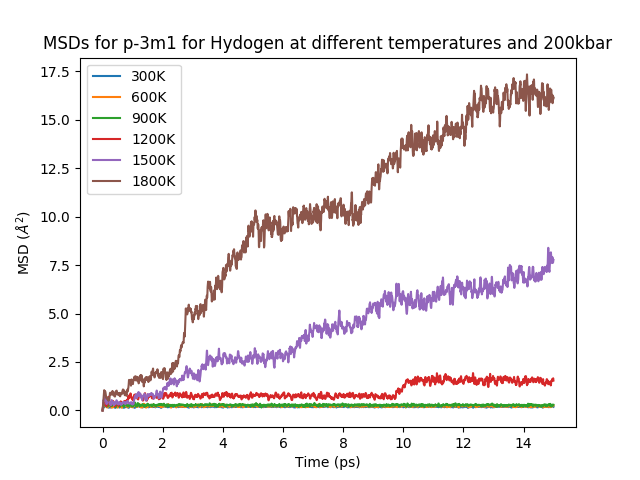
\includegraphics[width=7cm]{figures/p3m1_msd_H_p200.png}
	\subcaption{P$\bar{3}$m1 \SI{20}{\GPa}}
	\label{Fig8d}
\end{subfigure}%
\\
	\begin{subfigure}[t]{0.5\textwidth}
	\centering
	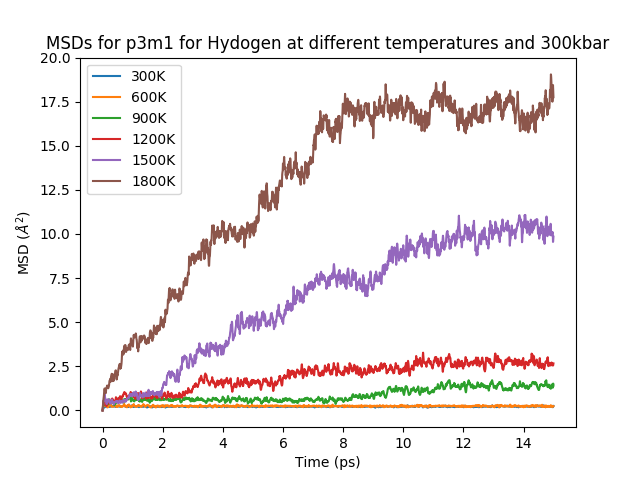
\includegraphics[width=7cm]{figures/p3m1_msd_H_p300.png}
	\subcaption{P$\bar{3}$m1 \SI{30}{\GPa}}
	\label{Fig8e}
\end{subfigure}%
	\caption{Brucite P$\bar{3}$m1 MSD results for hydrogen ions only}
	\label{Fig8}
\end{figure}

From this data it can be relatively easy to spot when superionicity is reached. This is seen when the line shoots off and the MSD value grows significantly. This will happen up to a point and then will reach a plateau due to the finite cell size. All the plots will show flucuations due to the ions moving around, however it is the gradient of the line which is the indicator if the ions are moving continuously further from their initial position. Moving large distances like this suggests the ions are free to move around and so the super-ionic state has been reached. A small step before returning to zero gradient in the MSD is an indication of some ions shifting along to a neighbouring oxygen, or swapping with a neighbouring hydrogen. This will increase the MSD slightly as they will be continuously further from their original position, but the zero gradient after means they are staying roughly at that distance and so the system is not superionic. This can be seen in the simulation done in VMD.

Beginning with the P$\bar{3}$m1 data, it suggests that the superionicity state for the hydrogen ions is not reached at \SI{1200}{\K} or below. This is due to the essentially zero gradient of all plots for these temperatures. In contrast, clear non zero gradients are seen for \SI{1500}{\K} and \SI{1800}{\K} at pressures \SI{20}{\GPa} and \SI{30}{\GPa}, and \SI{1800}{\K} for \SI{10}{\GPa}. These states are clearly super ionic due to the large gradients and reach over \SI{7.5}{\AA^2} MSD. However, for \SI{0}{\GPa} and \SI{5}{\GPa}, there are non zero gradient regions for \SI{1800}{\K}. Due to the MSD only reaching a max of roughly \SI{4}{\AA^2} and there being prolonged periods of constant MSD this is likely hydrogen ions shifting or swapping places and not being superionic (this is confirmed by studying the simulation in VMD).

\begin{table}[h!!]
	\centering
	\begin{tabular}{c|c|c|c|c|c|}
		\cline{2-6}
		& \SI{10}{\GPa} & \multicolumn{2}{c|}{\SI{20}{\GPa}} & \multicolumn{2}{c|}{\SI{30}{\GPa}} \\ \hline
		\multicolumn{1}{|c|}{}                                                             & \SI{1800}{\K}  & \SI{1500}{\K}        & \SI{1800}{\K}        & \SI{1500}{\K}        & \SI{1800}{\K}        \\ \hline
		\multicolumn{1}{|c|}{\begin{tabular}[c]{@{}c@{}}Diffusion\\ Constant\\ \SI{}{\AA^2\per\pico\second} \end{tabular}} & 0.230  & 0.123        & 0.291        & 0.216        & 0.460        \\ \hline
	\end{tabular}
	\caption{The diffusion constants for the superionic states of P$\bar3$m1.}
	\label{Tab1}
\end{table}

The diffusion constants for the superionic states of P$\bar3$m1 were calculated and are shown in Table 1. There is not much literature on diffusion constants for Brucite at these particular temperatures and pressures to compare the results. Instead, the proton diffusion constants of ice VII were calculated at similar pressures and 400K by Aoki \textit{et al} \cite{Aoki} and were found to be of the order of roughly \SI{1E-8}{\AA^2\per\pico\second}. This is much lower than the results in Table 1, suggesting a much more diffuse system in Brucite. However, the temperature difference of \SI{1400}{\K} is quite significant and a similar temperature for ice VII could make the results much more comparable.

\begin{figure}[h!!!!!!!!!!!!!!!!!!!!!!!!]
	\centering
	\begin{subfigure}[t]{0.5\textwidth}
		\centering
		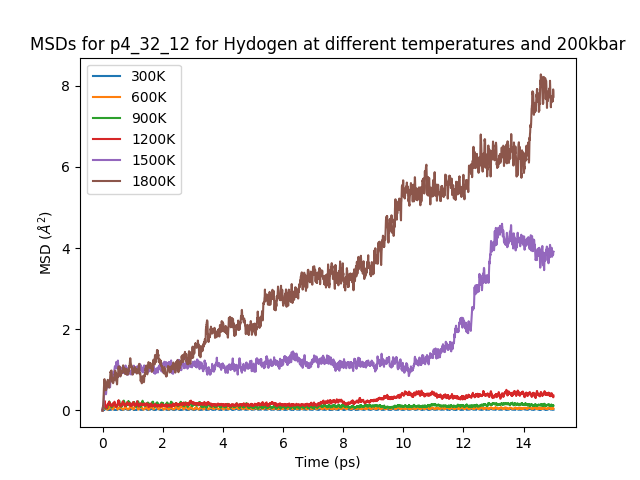
\includegraphics[width=6.5cm]{figures/p4_msd_H_p200.png}
		\subcaption{P4$_3$2$_1$2 \SI{20}{\GPa}}
		\label{Fig9a}
	\end{subfigure}%
	\begin{subfigure}[t]{0.5\textwidth}
		\centering
		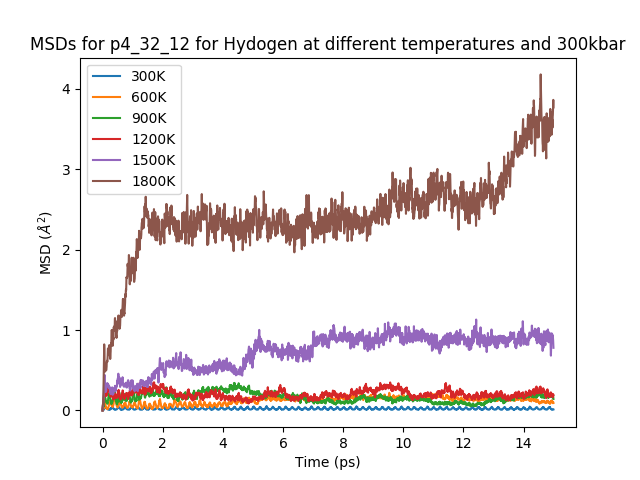
\includegraphics[width=6.5cm]{figures/p4_msd_H_p300.png}
		\subcaption{P4$_3$2$_1$2 \SI{30}{\GPa}}
		\label{Fig9b}
	\end{subfigure}%
	\\
	\begin{subfigure}[t]{0.5\textwidth}
		\centering
		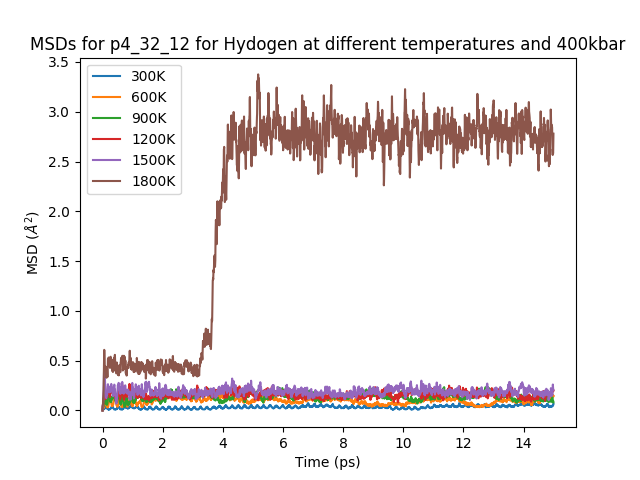
\includegraphics[width=6.5cm]{figures/p4_msd_H_p400.png}
		\subcaption{P4$_3$2$_1$2 \SI{40}{\GPa}}
		\label{Fig9c}
	\end{subfigure}%
	\caption{Brucite P4$_3$2$_1$2 MSD results for hydrogen ions only}
	\label{Fig9}
\end{figure}

Now looking at the P4$_3$2$_1$2 results, no superionic state appears to be achieved here. For all pressures, the data for \SI{1500}{\K} and below is all of roughly constant MSD (with flucuations). The exception is for \SI{20}{\GPa} and \SI{1500}{\K}, which has a relatively large jump in the MSD. There are also large jumps in all MSD data for \SI{1800}{\K} but then continuous MSD sections. For \SI{20}{\GPa}, the jumps are smaller in magnitude and happen over longer periods of time. There are single large jumps in \SI{30}{\GPa} and \SI{40}{\GPa}, the jump is notably larger and faster in the latter. To try and explain all these it is helpful to refer to the the structure of P4$_3$2$_1$2. Each hydrogen is bonded to an oxygen but extends towards another creating the zigzag patten. It is possible for the hydrogen ions to 'jump' to the opposite hydrogen and can cause a chain reaction of the hydrogens jumping across. For higher temperatures when the ions have more energy to move further and faster and at higher pressure the energy barrier is lower, these jumps can happen much quicker. This could explain these jumps and the correlation of their gradient with pressure and is confirmed when the simulations are studied.


\subsection{Hydrogen distribution and movement}

To get a clearer picture of some of the results from the MSD graphs, a hydrogen mapping programme and VMD were used to study the hydrogen ion distribution and simulation to look for things such hydrogen ions shifting or swapping sites.

\begin{figure}[h!!!!!!!!!!!!!!!!!!!!!]
	\centering
	\begin{subfigure}[t]{0.5\textwidth}
		\centering
		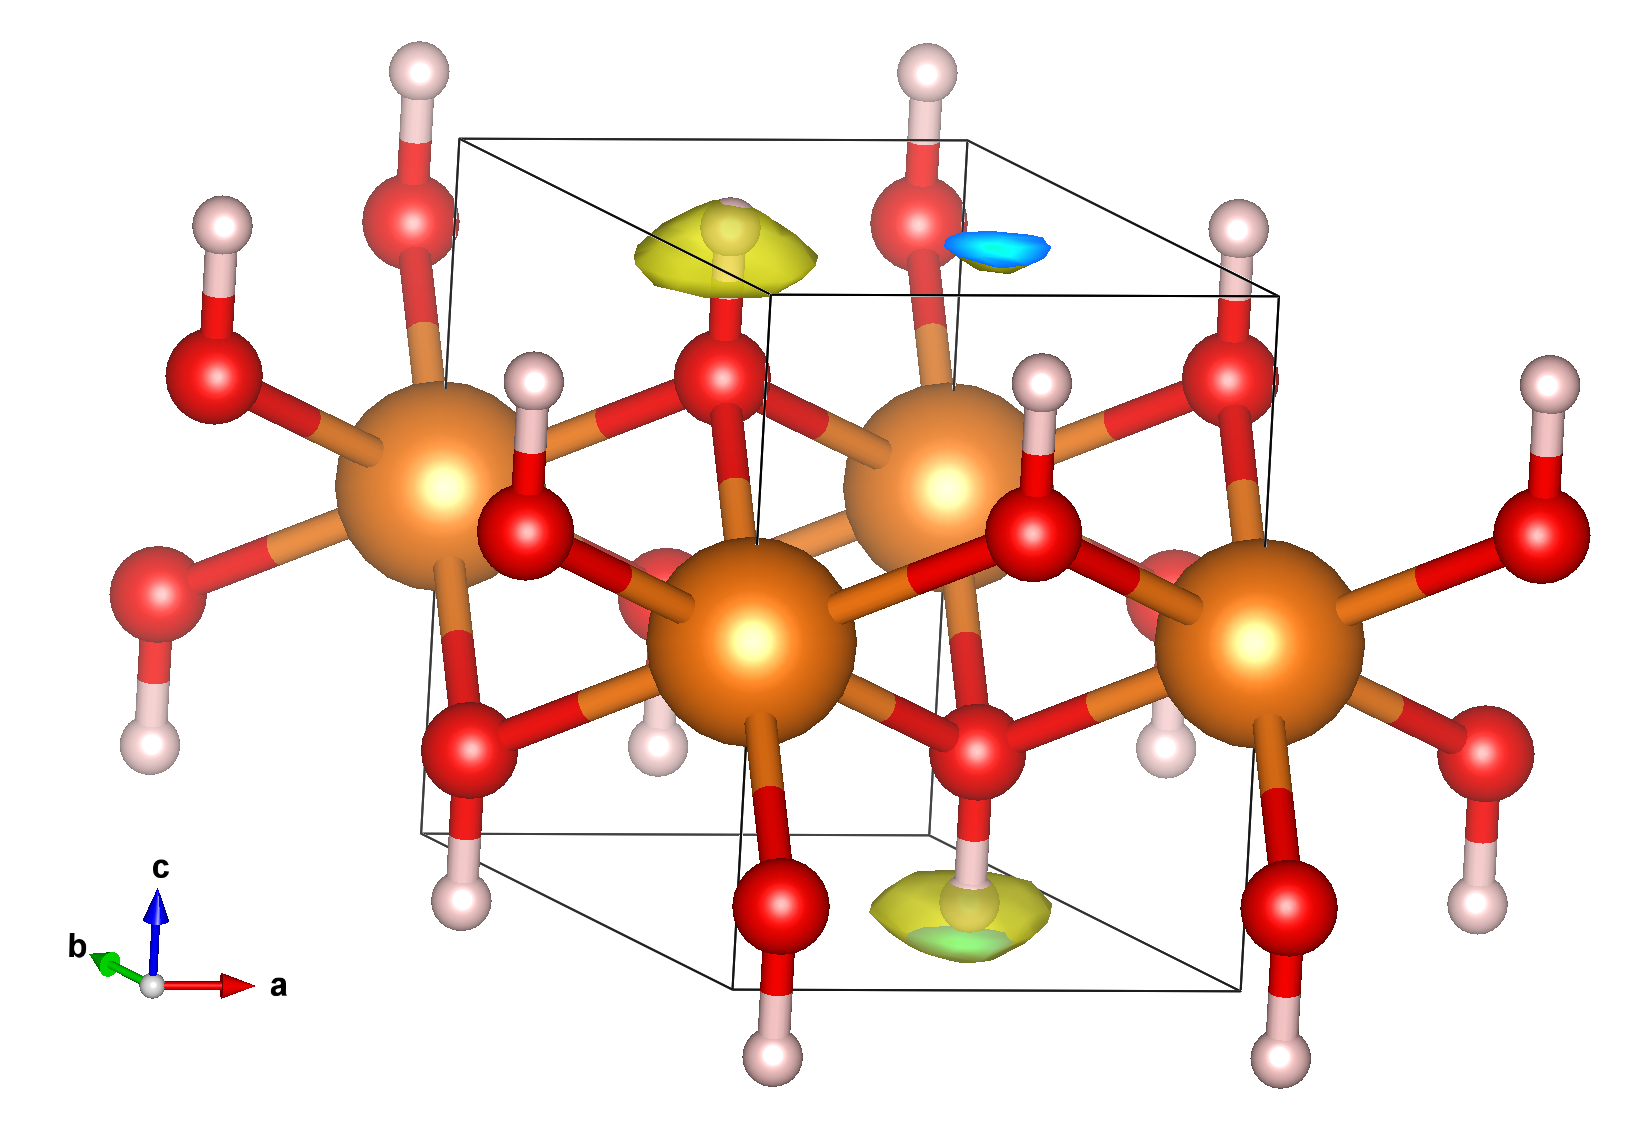
\includegraphics[width=7cm]{figures/p3_p0_t300_Hdist.png}
		\subcaption{P$\bar{3}$m1 \SI{0}{\GPa} \SI{300}{\K}}		
		\label{Fig10a}
	\end{subfigure}%
	\begin{subfigure}[t]{0.5\textwidth}
		\centering
		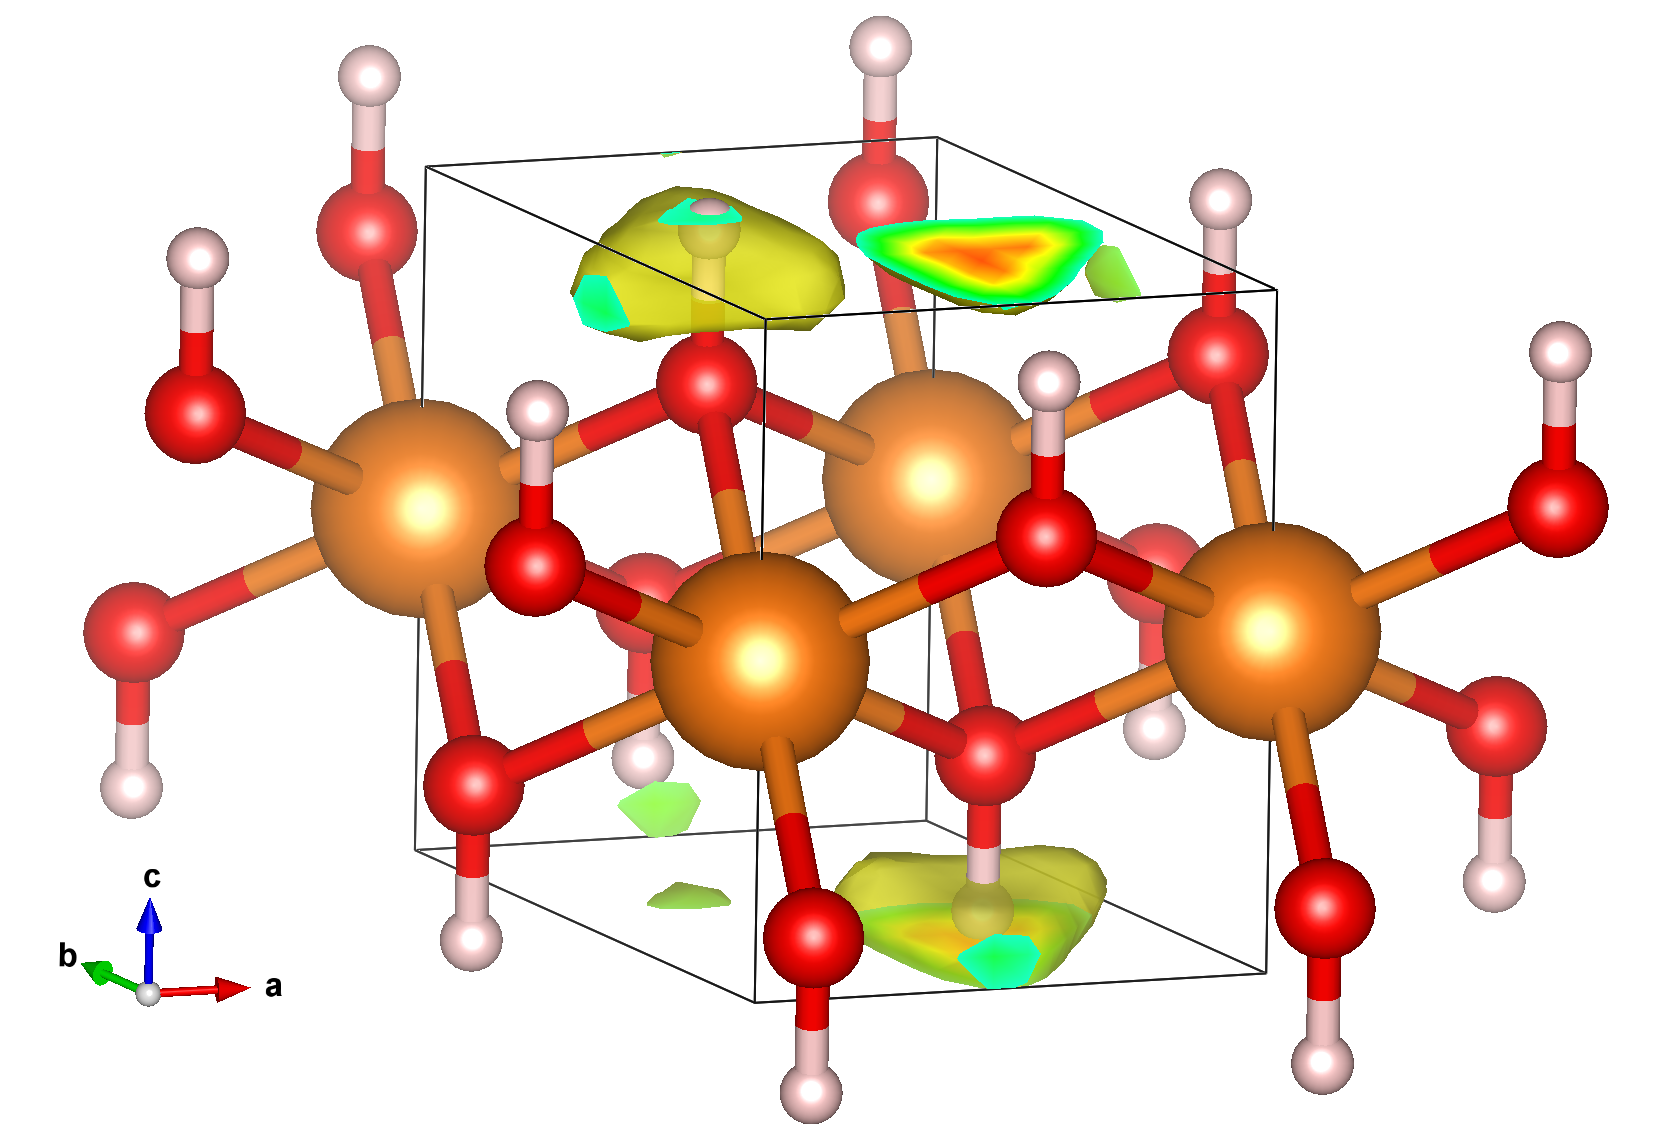
\includegraphics[width=7cm]{figures/p3_p100_t1800_Hdist.png}
		\subcaption{P$\bar{3}$m1 \SI{10}{\GPa} \SI{1800}{\K}}
		\label{Fig10b}
	\end{subfigure}%
	\\
	\begin{subfigure}[t]{0.5\textwidth}
		\centering
		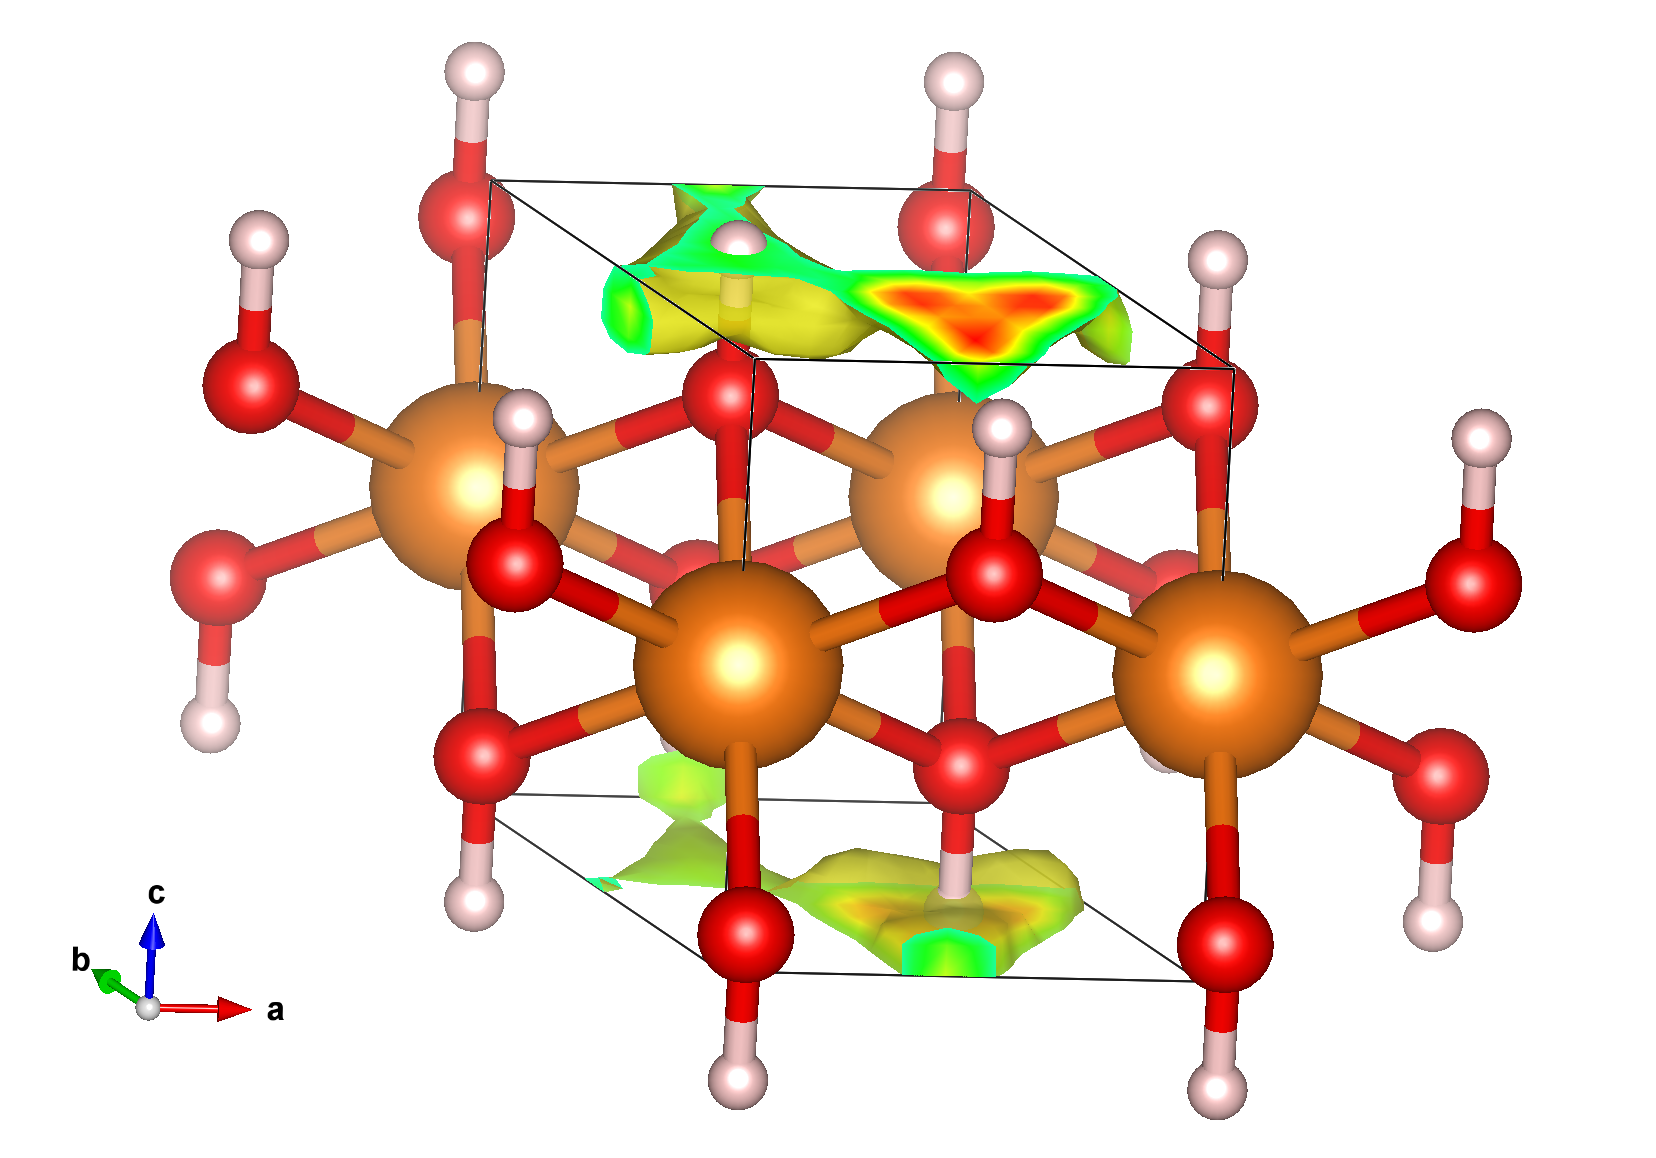
\includegraphics[width=7cm]{figures/p3_p300_t1800_Hdist.png}
		\subcaption{P$\bar{3}$m1 \SI{30}{\GPa} \SI{1800}{\K}}
		\label{Fig10c}
	\end{subfigure}%
	\\
	\begin{subfigure}[t]{0.5\textwidth}
		\centering
		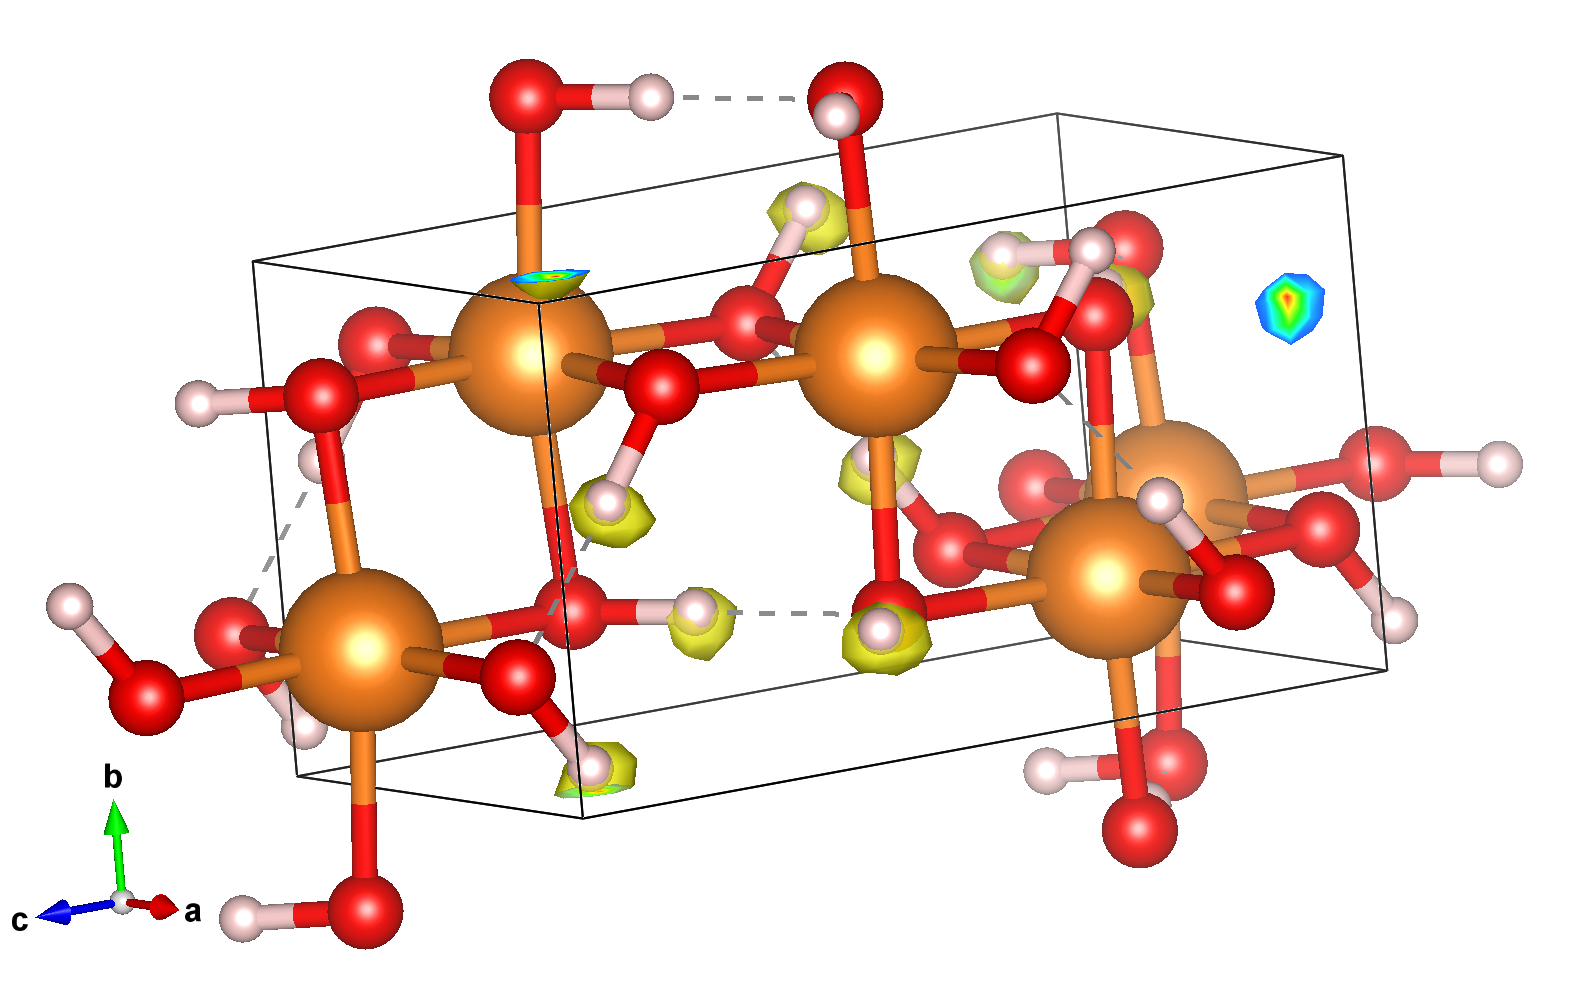
\includegraphics[width=7cm]{figures/p4_p200_t300_Hdist.png}
		\subcaption{P4$_3$2$_1$2 \SI{20}{\GPa} \SI{300}{\K}}		
		\label{Fig10d}
	\end{subfigure}%
	\begin{subfigure}[t]{0.5\textwidth}
		\centering
		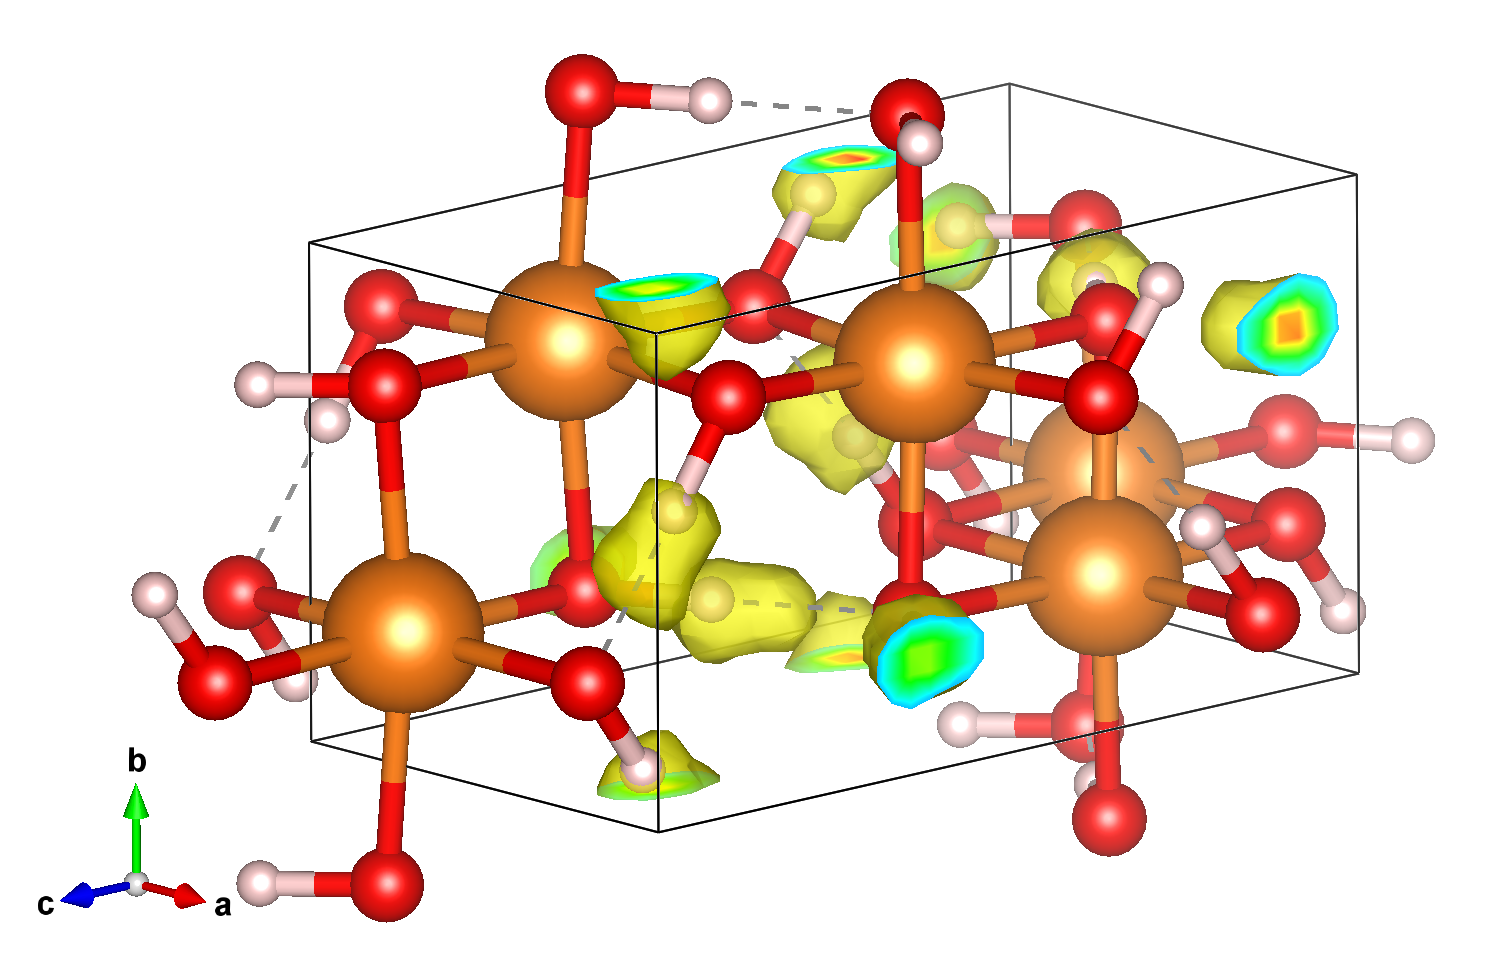
\includegraphics[width=7cm]{figures/p4_p200_t1800_Hdist.png}
		\subcaption{P4$_3$2$_1$2 \SI{20}{\GPa} \SI{1800}{\K}}
		\label{Fig10e}
	\end{subfigure}%
	\\
	\begin{subfigure}[t]{0.5\textwidth}
		\centering
		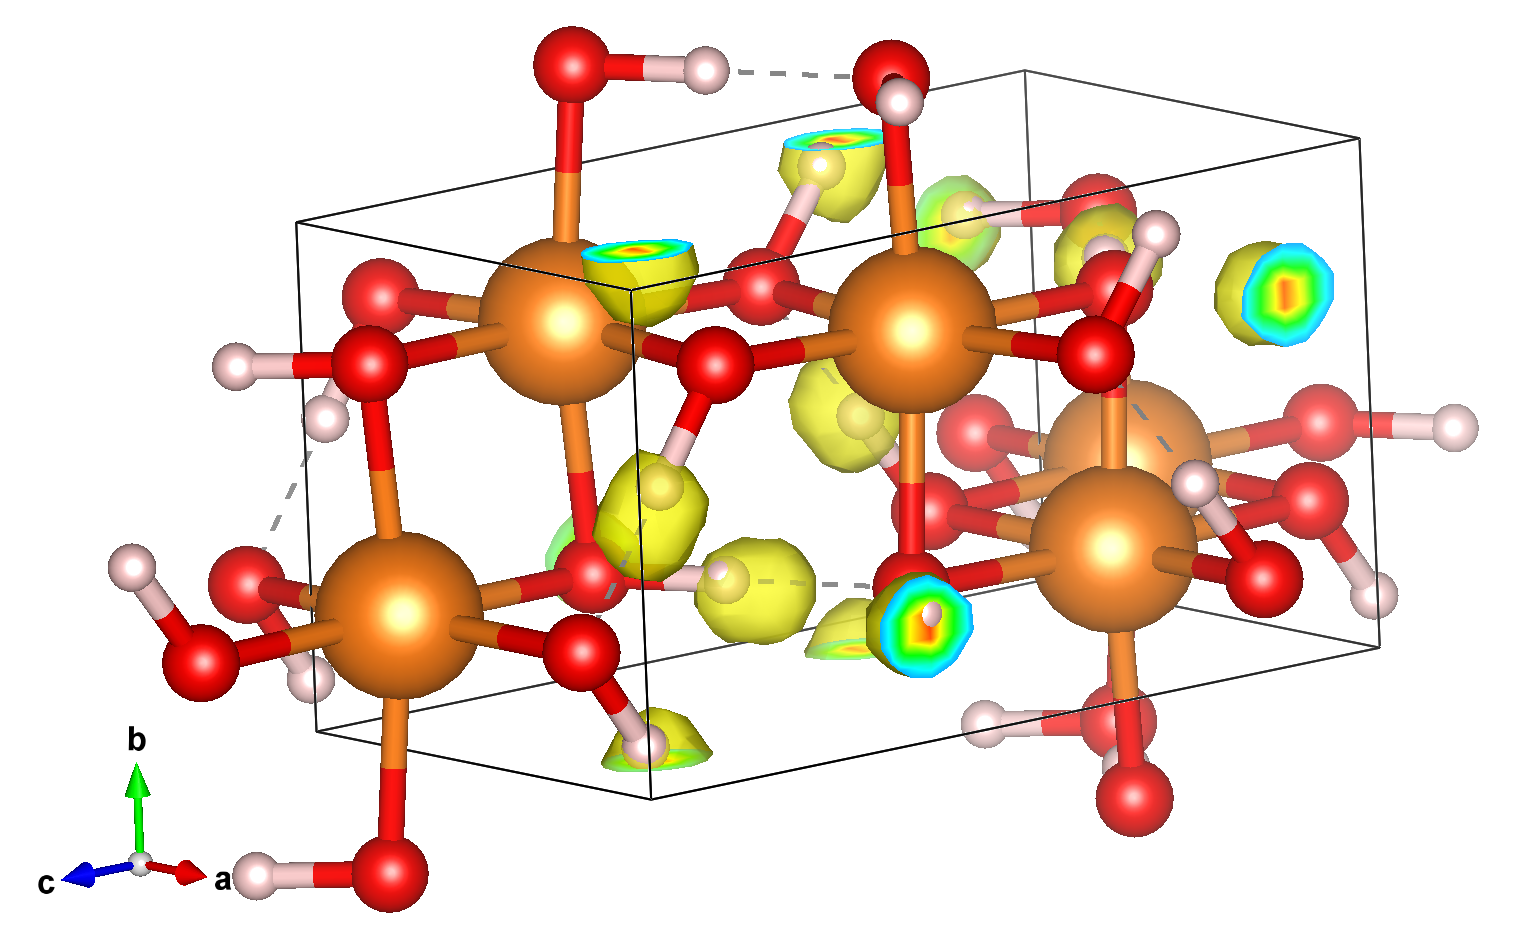
\includegraphics[width=7cm]{figures/p4_p400_t1800_Hdist.png}
		\subcaption{P4$_3$2$_1$2 \SI{40}{\GPa} \SI{1800}{\K}}
		\label{Fig10f}
	\end{subfigure}%
	\caption{Brucite P$\bar{3}$m1 and P4$_3$2$_1$2 hydrogen ion distributions as yellow isosurfaces mapped to the unit cell. Produced using VESTA.}
	\label{Fig10}
\end{figure}

Some examples of the hydrogen distributions mapped to the unit cell have been included here in Figure \ref{Fig10} to verify some of the observations mentioned in the previous section. It is clear that as temperature increases the hydrogen ions move much more freely in the layer of the P$\bar{3}$m1 phase.  Both \SI{10}{\GPa} and \SI{30}{\GPa} pressures are superionic states and can be seen by the large almost free areas they are free to move around. For the P4$_3$2$_1$2 phase, larger areas of movement for the hydrogens are expected (as the protons have more energy to move) and shown and no superionic state is seen, as expected. However, these images do not explain the large jumps seen in the MSD graphs. Instead an image from VMD is shown in Figure \ref{Fig11}.

\begin{figure}[h!!!!!!!!]
	\centering
	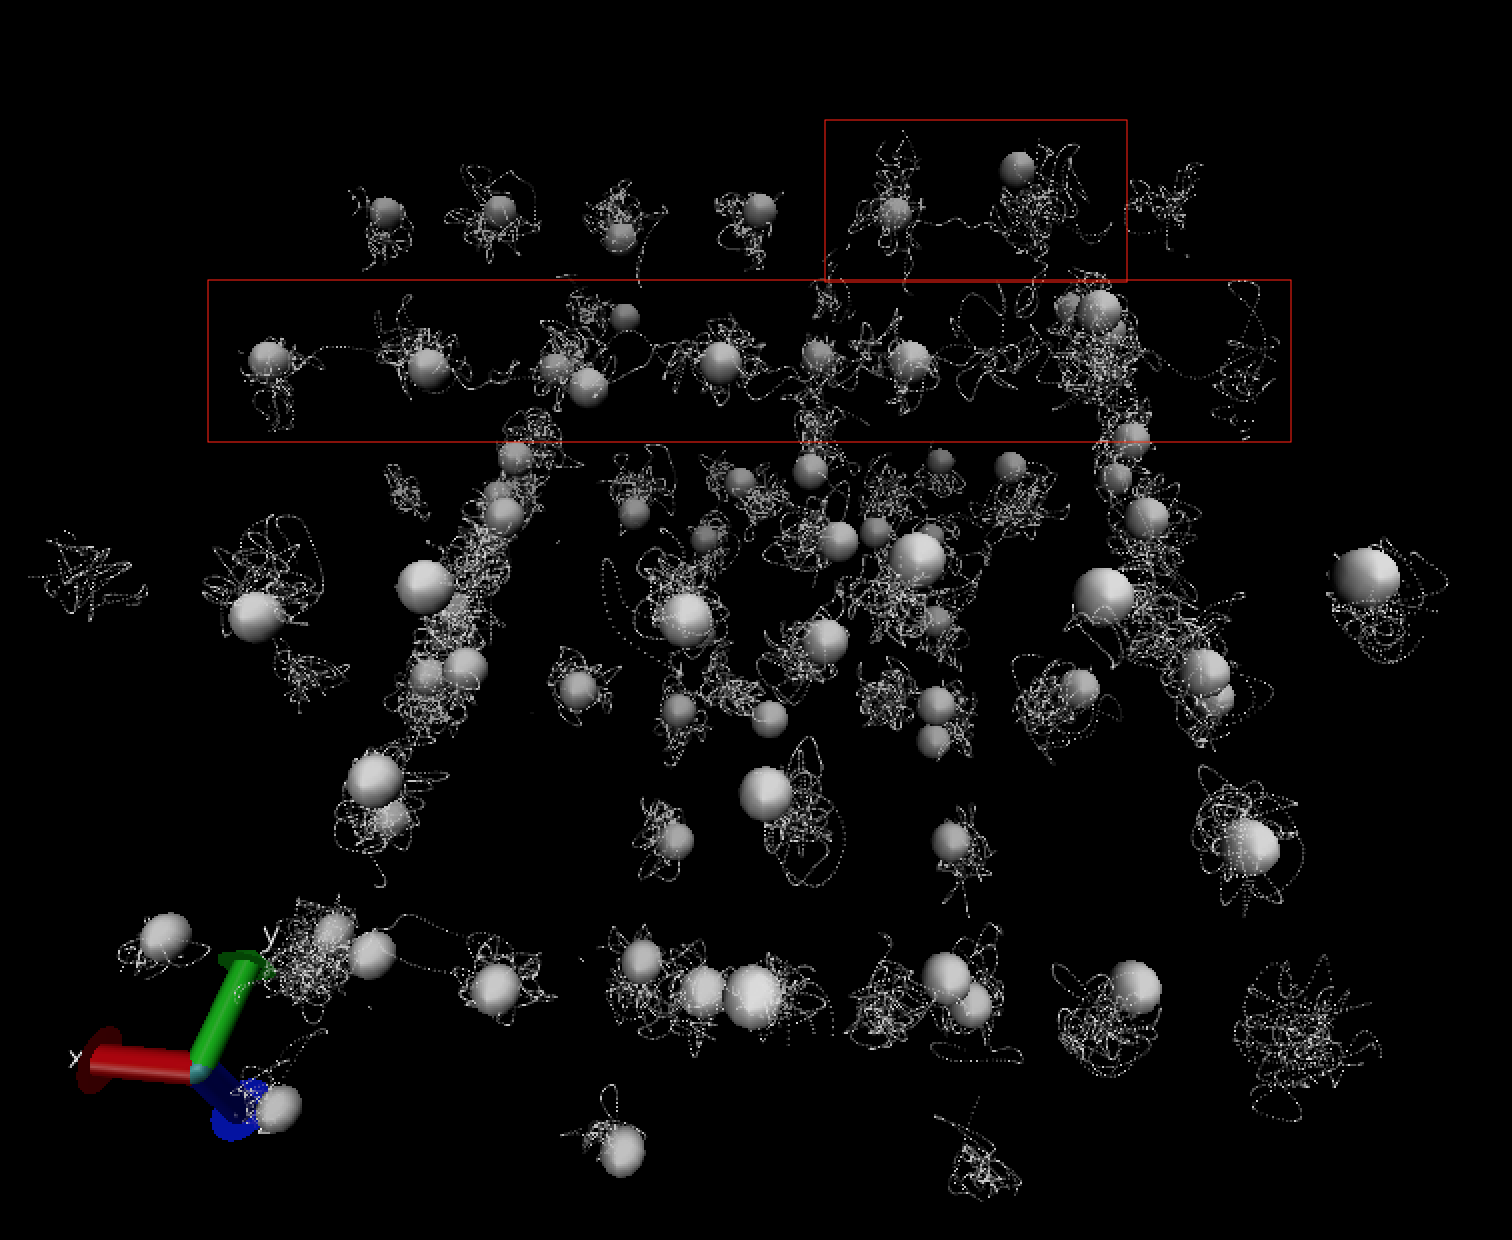
\includegraphics[width=11cm]{figures/vmd_p4_p400_t1800.png}
	\caption{An image from the VMD simulation showing only the hydrogen atoms positions throughout the 3.5-\SI{4.5}{\pico\second} interval for the P4$_3$2$_1$2 phase at \SI{40}{\GPa} and \SI{1800}{\K}. The large white spheres are the orginal positions and the small white points are the positions at every timestep in the interval. The red outlines show areas where swapping and shifting of the hydrogen ions has occured.}
	\label{Fig11}
\end{figure}

Figure \ref{Fig11} shows only the hyrdogen ions in the P$4_32_12$ phase in the time interval represented the large jump in MSD for \SI{400}{\GPa} and \SI{1800}{\K}. In the highlighted areas, trails of the hydrogen ions shifting along the sites and swapping between sights can be seen (this may be difficult as they are smaller points). Many of these occurences cause the large jumps in MSD as seen previously. This is an example of how the simulation shows the anticipated jumps and swaps leading to the MSD increases.

\newpage
\subsection{RDF and PDF}

The RDF and PDF graphs can also be used to provide structural and ordering information on the simulation. Figures \ref{Fig12} and \ref{Fig13} show the RDFs and PDFs for the OH and MgO bonds at various temperatures and pressures for the P$\bar3$m1 and P$4_32_12$ phases respectively. It is worth noting that the PDF scale appears to be slightly off for the OH graphs, however this won't affect the shape too much and the data is still useable for comparison.

\begin{figure}[h!!!!!!!!!!!!]
	\centering
		\begin{subfigure}{0.32\textwidth}
		\centering
		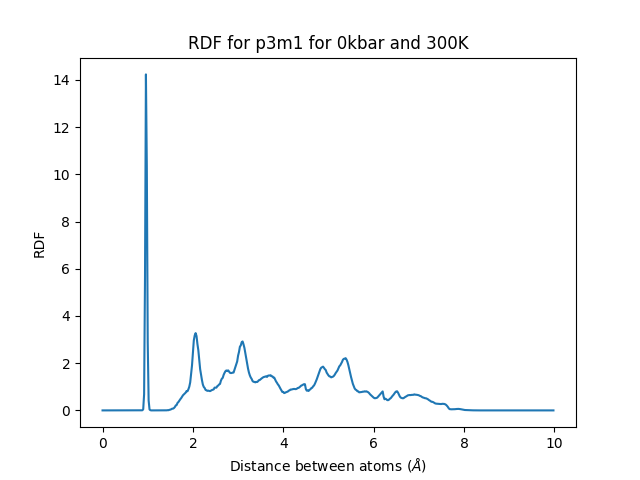
\includegraphics[width=5.5cm]{figures/p3_rdf_p0_t300.png}
		\subcaption{P$\bar3$m1 \SI{0}{\GPa} \SI{300}{\K} RDF}
		\label{Fig12a}
	\end{subfigure}%
	\begin{subfigure}{0.32\textwidth}
		\centering
		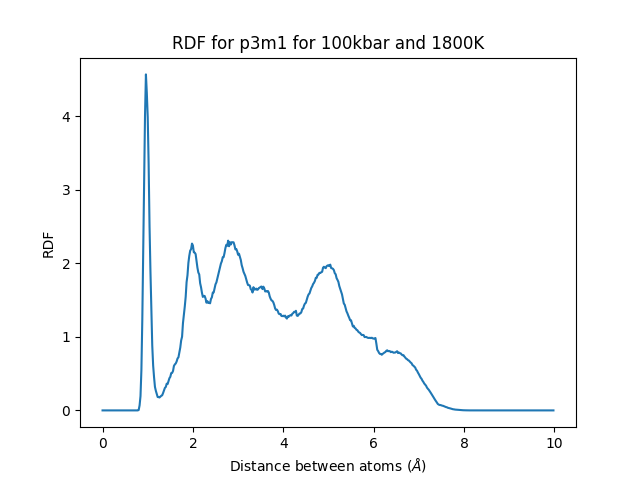
\includegraphics[width=5.5cm]{figures/p3_rdf_p100_t1800.png}
		\subcaption{P$\bar3$m1 \SI{10}{\GPa} \SI{1800}{\K} RDF}
		\label{Fig12b}
	\end{subfigure}%
	\begin{subfigure}{0.32\textwidth}
	\centering
	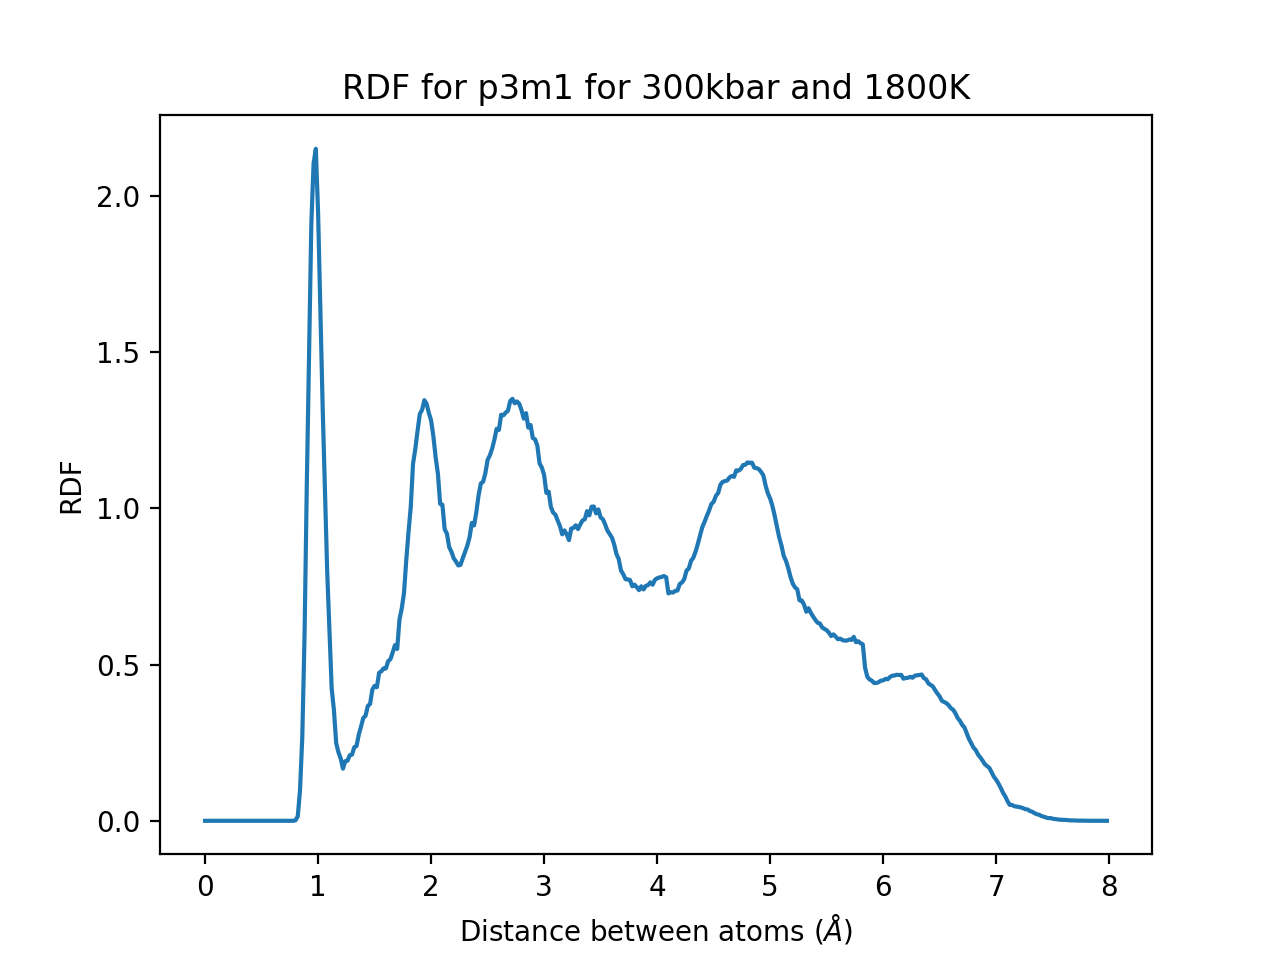
\includegraphics[width=5.5cm]{figures/rdfp3p300t1800c100.png}
	\subcaption{P$\bar3$m1 \SI{30}{\GPa} \SI{1800}{\K} RDF}
	\label{Fig12c}
\end{subfigure}%
\\
	\begin{subfigure}{0.32\textwidth}
	\centering
	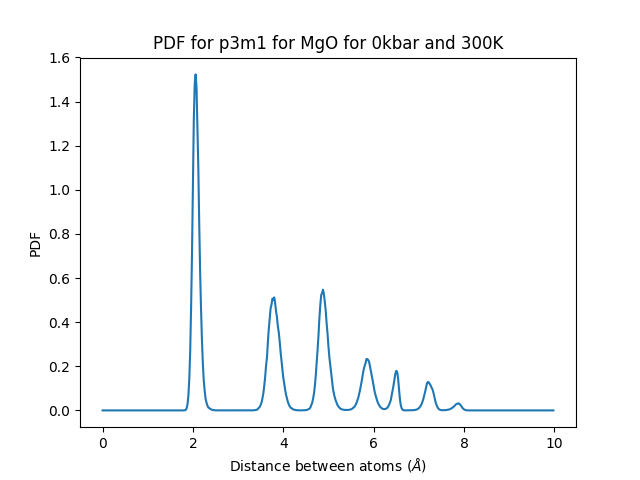
\includegraphics[width=5.5cm]{figures/p3_pdf_MgO_p0_t300.png}
	\subcaption{P$\bar3$m1 \SI{0}{\GPa} \SI{300}{\K} MgO PDF}
	\label{Fig12d}
\end{subfigure}%
	\begin{subfigure}{0.32\textwidth}
	\centering
	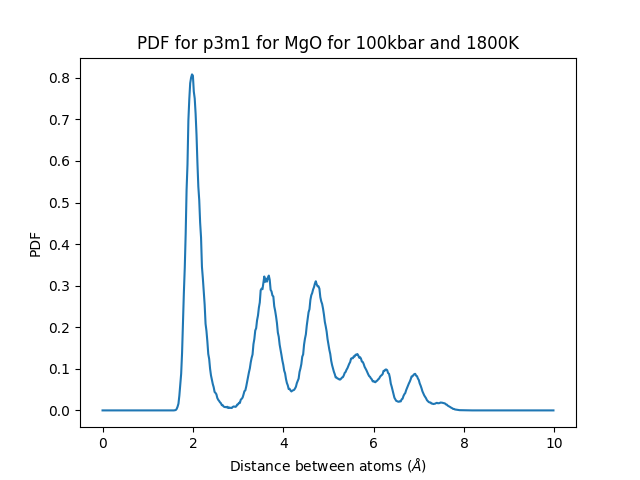
\includegraphics[width=5.5cm]{figures/p3_pdf_MgO_p100_t1800.png}
	\subcaption{P$\bar3$m1 \SI{10}{\GPa} \SI{1800}{\K} MgO PDF}
	\label{Fig12e}
\end{subfigure}%
	\begin{subfigure}{0.32\textwidth}
	\centering
	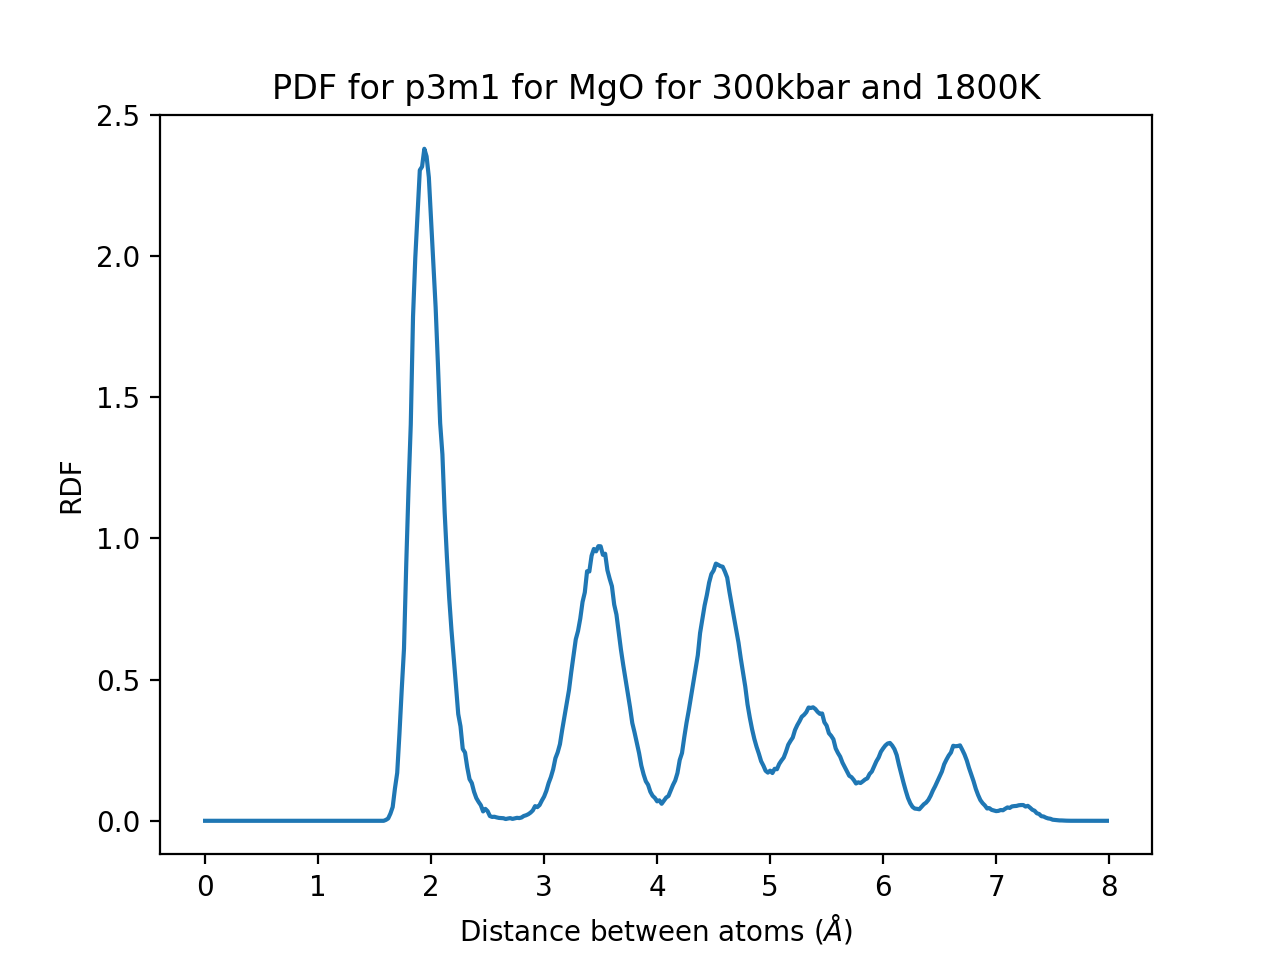
\includegraphics[width=5.5cm]{figures/pdfMgOp3p300t1800c100.png}
	\subcaption{P$\bar3$m1 \SI{30}{\GPa} \SI{1800}{\K} MgO PDF}
	\label{Fig12f}
\end{subfigure}%
\\	
\begin{subfigure}{0.32\textwidth}
	\centering
	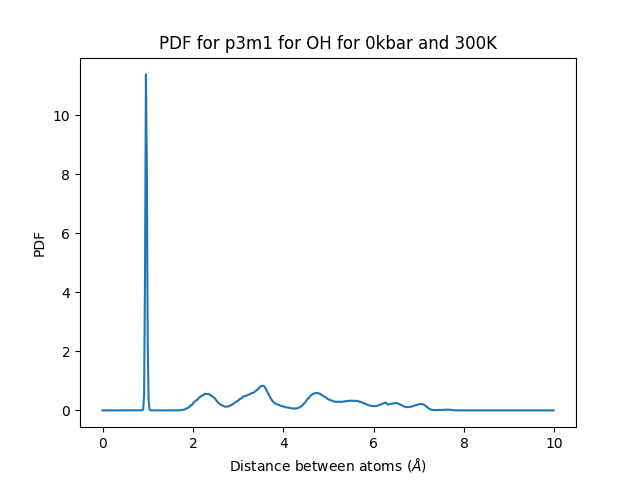
\includegraphics[width=5.5cm]{figures/p3_pdf_OH_p0_t300.png}
	\subcaption{P$\bar3$m1 \SI{0}{\GPa} \SI{300}{\K} OH PDF}
	\label{Fig12g}
\end{subfigure}%
\begin{subfigure}{0.32\textwidth}
	\centering
	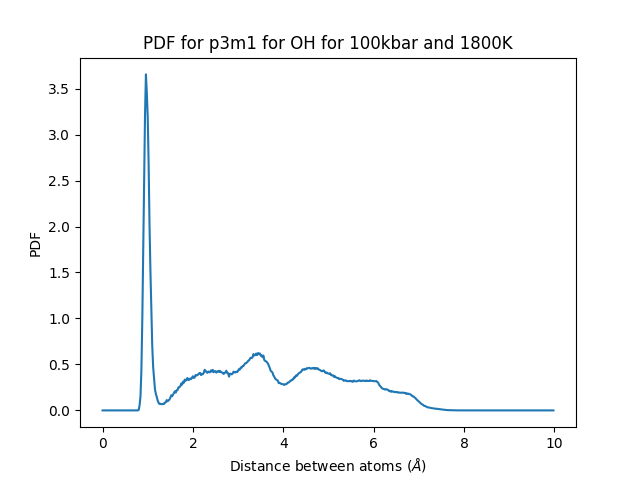
\includegraphics[width=5.5cm]{figures/p3_pdf_OH_p100_t1800.png}
	\subcaption{P$\bar3$m1 \SI{10}{\GPa} \SI{1800}{\K} OH PDF}
	\label{Fig12h}
\end{subfigure}%
	\begin{subfigure}{0.32\textwidth}
	\centering
	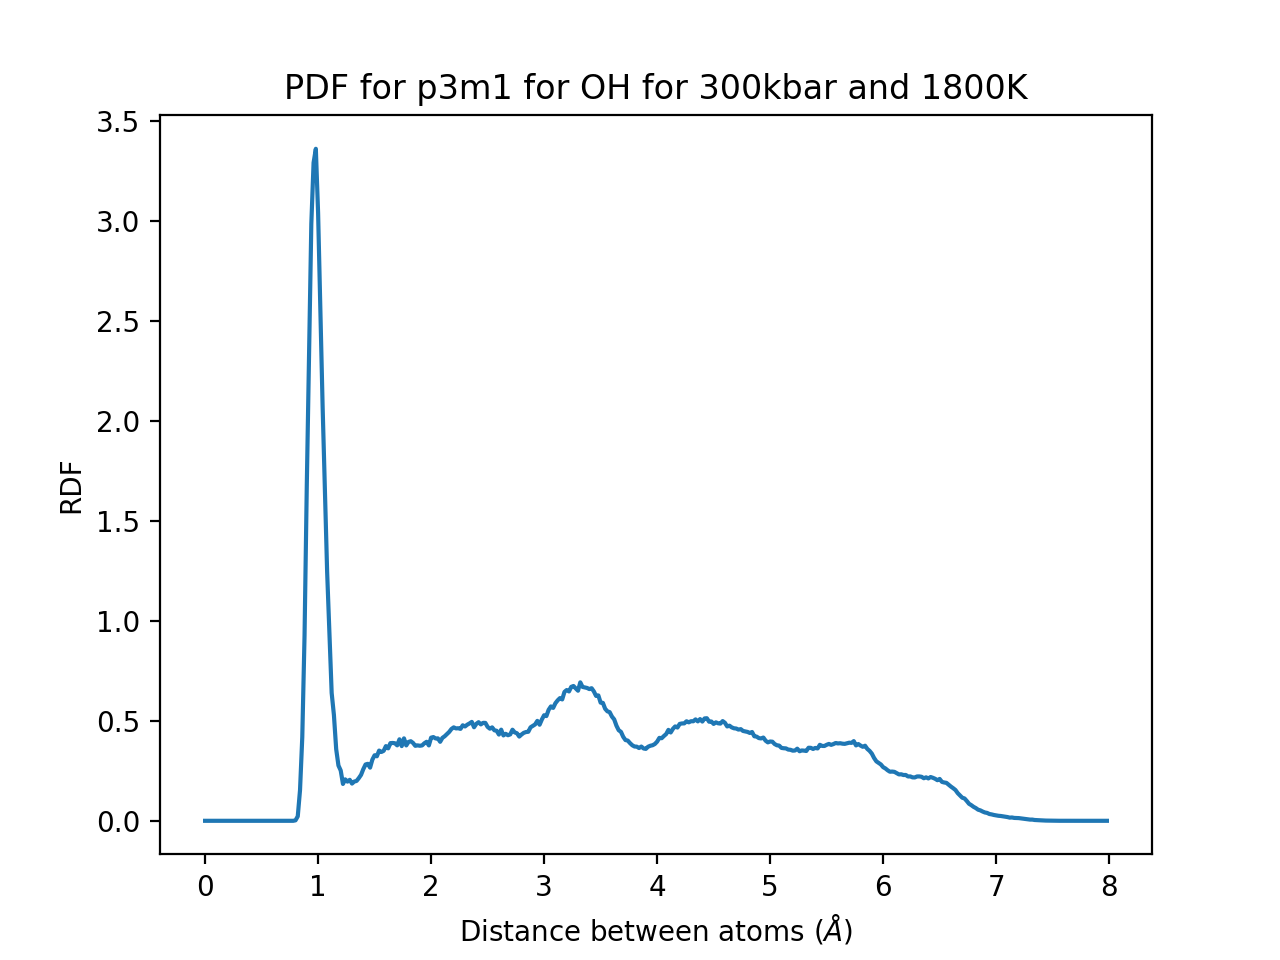
\includegraphics[width=5.5cm]{figures/pdfOHp3p300t1800c100.png}
	\subcaption{P$\bar3$m1 \SI{30}{\GPa} \SI{1800}{\K} OH PDF}
	\label{Fig12i}
\end{subfigure}%
\caption{The RDF and PDFs of the MgO and OH bonds for the P$\bar3$m1 phase at \SI{0}{\GPa} \SI{300}{\K}, \SI{10}{\GPa} \SI{1800}{\K} and \SI{30}{\GPa} \SI{1800}{\K}.}
\label{Fig12}
\end{figure}

\begin{figure}[h!!!!!!!!!!]
	\centering
	\begin{subfigure}{0.32\textwidth}
		\centering
		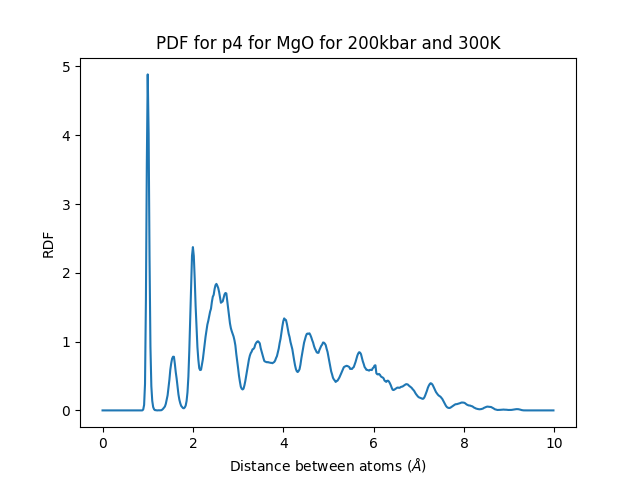
\includegraphics[width=5.5cm]{figures/p4_rdf_p200_t300.png}
		\subcaption{P$4_32_12$ \SI{20}{\GPa} \SI{300}{\K} RDF}
		\label{Fig13a}
	\end{subfigure}%
	\begin{subfigure}{0.32\textwidth}
		\centering
		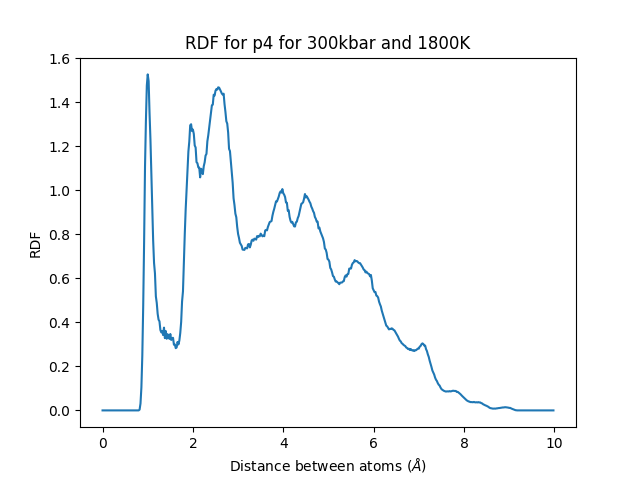
\includegraphics[width=5.5cm]{figures/p4_rdf_p300_t1800.png}
		\subcaption{P$4_32_12$ \SI{30}{\GPa} \SI{1800}{\K} RDF}
		\label{Fig13b}
	\end{subfigure}%
	\begin{subfigure}{0.32\textwidth}
		\centering
		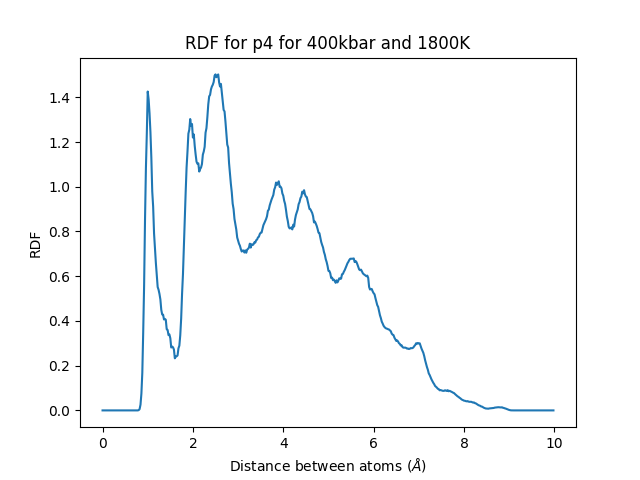
\includegraphics[width=5.5cm]{figures/p4_rdf_p400_t1800.png}
		\subcaption{P$4_32_12$ \SI{40}{\GPa} \SI{1800}{\K} RDF}
		\label{Fig13c}
	\end{subfigure}%
	\\
	\begin{subfigure}{0.32\textwidth}
		\centering
		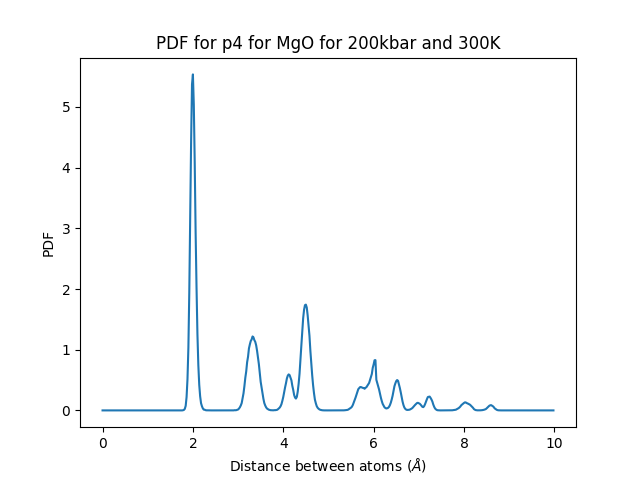
\includegraphics[width=5.5cm]{figures/p4_pdf_MgO_p200_t300.png}
		\subcaption{P$4_32_12$ \SI{20}{\GPa} \SI{300}{\K} MgO PDF}
		\label{Fig13d}
	\end{subfigure}%
	\begin{subfigure}{0.32\textwidth}
		\centering
		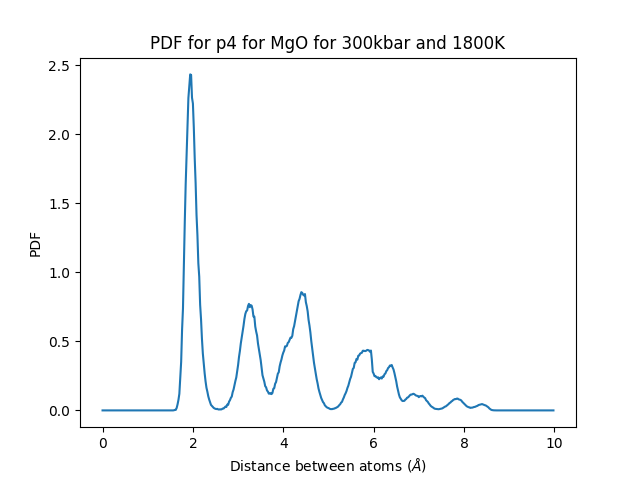
\includegraphics[width=5.5cm]{figures/p4_pdf_MgO_p300_t1800.png}
		\subcaption{P$4_32_12$ \SI{30}{\GPa} \SI{1800}{\K}MgO PDF}
		\label{Fig13e}
	\end{subfigure}%
	\begin{subfigure}{0.32\textwidth}
		\centering
		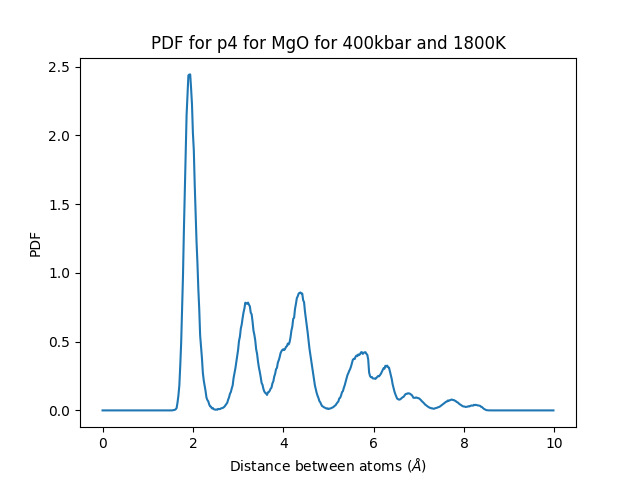
\includegraphics[width=5.5cm]{figures/p4_pdf_MgO_p400_t1800.png}
		\subcaption{P$4_32_12$ \SI{40}{\GPa} \SI{1800}{\K} MgO PDF}
		\label{Fig13f}
	\end{subfigure}%
	\\	
	\begin{subfigure}{0.32\textwidth}
		\centering
		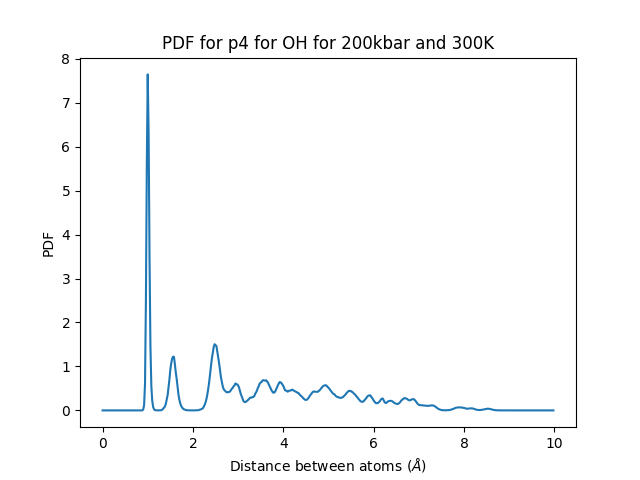
\includegraphics[width=5.5cm]{figures/p4_pdf_OH_p200_t300.png}
		\subcaption{P$4_32_12$ \SI{20}{\GPa} \SI{300}{\K} OH PDF}
		\label{Fig13g}
	\end{subfigure}%
	\begin{subfigure}{0.32\textwidth}
		\centering
		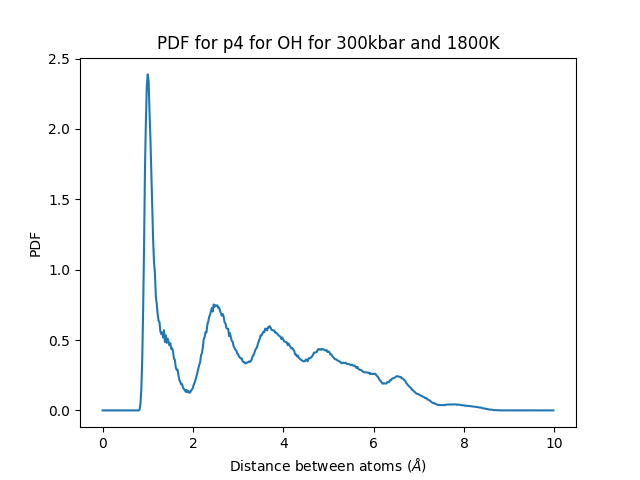
\includegraphics[width=5.5cm]{figures/p4_pdf_OH_p300_t1800.png}
		\subcaption{P$4_32_12$ \SI{30}{\GPa} \SI{1800}{\K} OH PDF}
		\label{Fig13h}
	\end{subfigure}%
	\begin{subfigure}{0.32\textwidth}
		\centering
		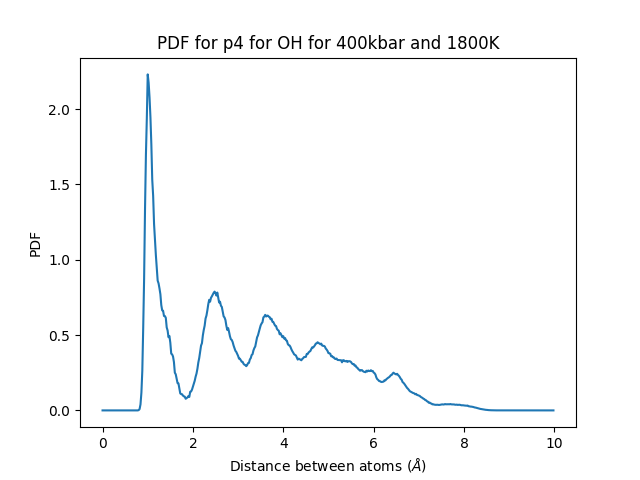
\includegraphics[width=5.5cm]{figures/p4_pdf_OH_p400_t1800.png}
		\subcaption{P$4_32_12$ \SI{40}{\GPa} \SI{1800}{\K}OH PDF}
		\label{Fig13i}
	\end{subfigure}%
	\caption{The RDF and PDFs of the MgO and OH bonds for the P$4_32_12$ phase at \SI{20}{\GPa} \SI{300}{\K}, \SI{30}{\GPa} \SI{1800}{\K} and \SI{40}{\GPa} \SI{1800}{\K}.}
	\label{Fig13}
\end{figure}

For the P$\bar3$m1 data in Figure \ref{Fig12}, the \SI{0}{\GPa} and \SI{300}{\K} state shows the RDF and PDFs for a known solid state. The \SI{30}{\GPa} \SI{1800}{\K} state is known to be superionic as seen from the MSD and hydrogen ion distribution data. These can both be used as comparisons to study the \SI{10}{\GPa} \SI{1800}{\K} state presumed to be superionic from the previous data. The RDF graphs for the low pressure phase show a solid shape, with some movement of the constituent ions creating the less sharp peaks after the intial spike. The middle and higher pressure states have a liquid shape in the graph as seen by the large peak at one with some smaller peaks after that are comparable in size to the initial peak. The tail off towards the end of these graphs is a feature due to the finite cell size of the system. The liquid shape suggests some of the ions are much more mobile and fluid like.

The PDFs for MgO all show a very solid structure with a series of well defined peaks. This shows the Mg and O ions maintain their structure and do not  become more fluid like. However, the PDF for OH is in stark contrast to this. It shows a very fluid like structure for the higher pressure and temperature phases by the indistinguished peaks after the large initial peak. The \SI{0}{\GPa} \SI{300}{\K} phase has a much smaller 'mound' after the initial peak and represents the more bound hydrogen states, which have less energy and freedom to move around in the cell. Seeing the many similarities of the \SI{10}{\GPa} \SI{1800}{\K} state with the superionic state, this provides further evidence for it being superionic also.

The P$4_32_12$ results in Figure \ref{Fig13} all appear to give the same overall trend. The \SI{20}{\GPa} \SI{300}{\K} phase has much lower successive peaks due to the ions having less energy to move around although its overall shape is similar to the higher pressure and temperature phases. all three show a solid structure with a series of noticeable peaks. Particularly, the OH PDF shows much more established peaks in contrast to the superionic OH PDFs of the P$\bar3$m1 phase, providing evidence for the conclusion that no superionic state of the P$4_32_12$ phase is reached.

\subsection{Pressure-temperature graph}

Using all of this collected data an approximate pressure-temperature (PT) graph can be produced, as shown in Figure \ref{PT}.

\begin{figure}[h!!!!!!!!]
	\centering
	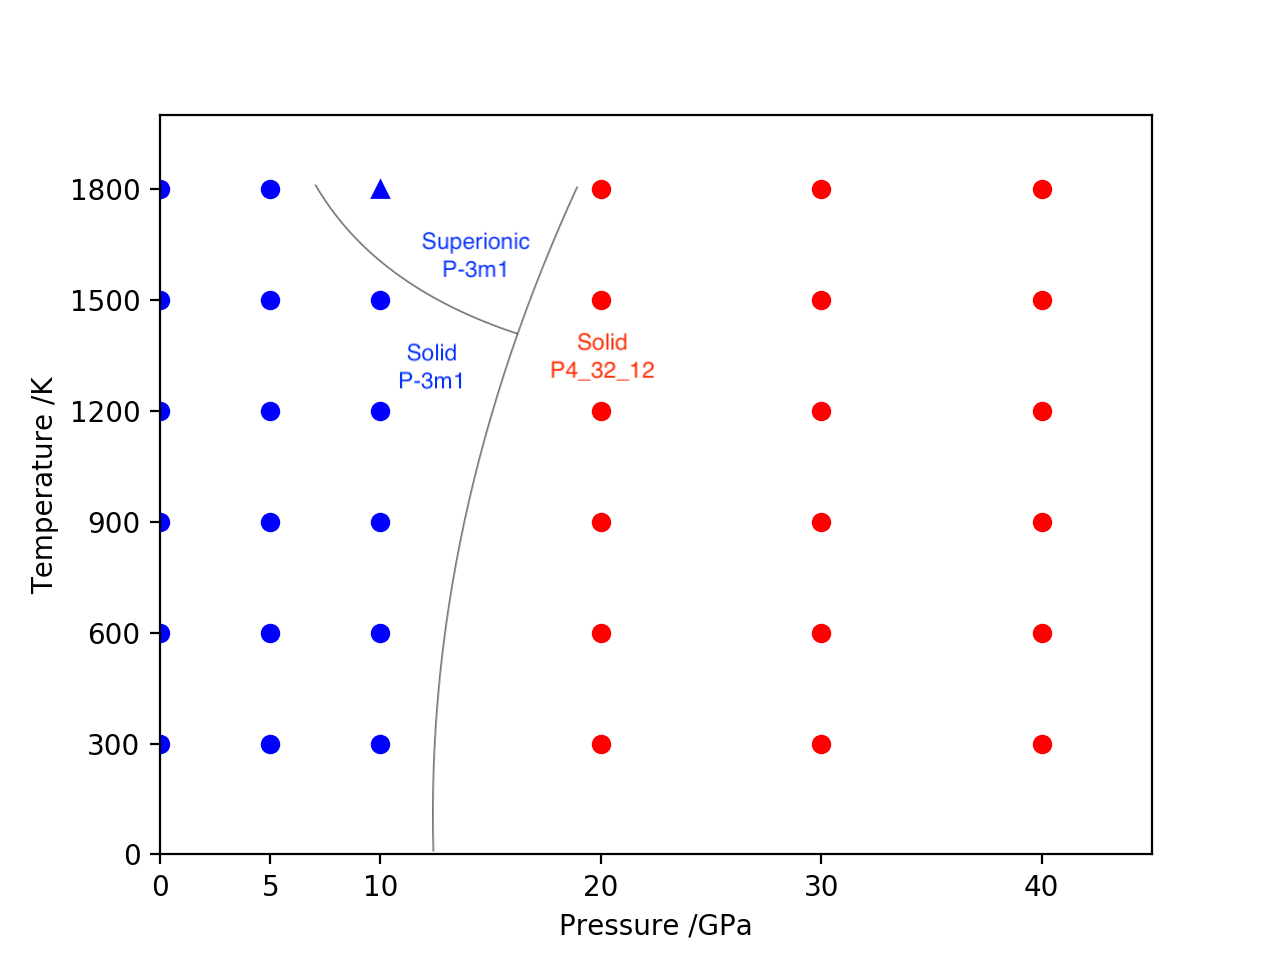
\includegraphics[width=11cm]{figures/PT_graph.png}
	\caption{An estimated PT diagram of Brucite. The phase boundary is hand drawn by estimation using the data gathered in the project. The triple point is also highly estimated. Blue circles represent solid P$\bar3$m1, blue triangles represent superionic P$\bar3$m1 and red circles represent solid P4$_32_12$ and are all pressure-temperature points MD was carried out at.}
	\label{PT}
\end{figure}

The points on the graph are the points at which MD was carried out. The pressures should all be slightly higher than presented (magnitude of difference increases with temperature) as the MD simulations are actually carried out at a pressure slightly above the optimised pressure. However, to save time and space on the data output of the simulations, the settings were turned down and consequently the actual pressure of the MD was not written out. This is a point to improve on if the project were to be repeated as  it would give a slightly more accurate PT graph. 

The \SI{0}{\K} transition point was chosen as roughly \SI{12}{\GPa} due to the reuslts of the structure optimisation energy differences. The individual points were decided as solid or superionic based on the MSD, hydrogen distributions, simulations and the PDFs and RDFs. From here the phase boundaries can be estimated along with the triple pointbased on their positions. These are very rough estimates due to the low density of points calculated on the grid, but give a rough overview of shape and structure of the actual PT graph.

\bigskip

\noindent To improve the results, the actual pressure of the MD simulations could also be output to produce a more accurate PT graph, as the operating pressure of the MD is actually slightly above the pressure that the optimised structures were found at. The normalisation of the PDF graphs could also be fixed. More data could be gathered to create a more dense grid for the PT diagram providing a more accurate picture. Analysis on the errors created by the chosen settings, such as the plane wave cut-off energy, could be done to provide an estimation of the error on the obtained results. Other implementations of DFT (such as different functionals) could also be implemented to compare results and see if they are in agreement or a more accurate solution could be found. A larger cell could also be used to reduce the correlation. Using a large enough cell and at high enough temperatures and pressures may also allow decomposition to be studied, although this would need to be paritcularly large. One possibility is to make the cell signifcantly longer in one direction only, to act as a 'slice' of a macroscopic crystal. This would allow the water molecules to split from MgO molecules. However, this is not a certainty and is quite difficult to achieve in MD. Finally, the simulations could be carried out for other hydrous compounds from the mantle to compare the results. This would offer more insight into water transportation in the mantle and the effectiveness of certain compounds at water transportation.

From these results it can be seen that the P$4_32_12$ phase is stable at higher pressures and temperatures than the P$\bar3$m1 phase and so would be expected to be found deeper in the mantle at these higher pressures and temperatures. This allows Brucite to transport water over a significant depth in the mantle and suggests it is highly active in this role. Given other mineral studies similar to this the transport cycle in the mantle could become very well undertsood.
 
 
\section{Conclusion}
%
%This section should summarise the results obtained, detail
%conclusions reached, suggest future work, and changes that you would make if you repeated the
%experiment. This section should in general be short, 100 to 150 words
%being typical for most projects.
%\par\noindent
%If you have opted to have multiple {\bf Theory, Method, Results}
%sections, draw all the results together in a {\bf single} conclusion.
The initial energy of optimised states graph suggested a phase change at around \SI{12}{\GPa}. At \SI{1800}{\K} and \SI{10}{\GPa} the P$\bar3$m1 phase was found to be superionic with the hydrogen ions free to move around in the layer between Mg and O layers. This was found via the MSD results and was confirmed with the RDF and PDFs and the hydrogen distribution viewing techniques. As expected, states at \SI{1500}{\K} and above at pressures above \SI{12}{\GPa} were also found to be superionic in P$\bar3$m1 and this was used to confirm the superionicity of the \SI{10}{\GPa} \SI{1800}{\K} state. The diffusion constants of the these states were of the order of \SI{0.1}{\AA^2\per\pico\second}, much higher than ice VII at similar pressures but a significantly lower temperature of \SI{400}{\K}. P$4_32_12$ was found to be solid at 20-\SI{40}{\GPa} and up to \SI{1800}{\K} by the same techniques. A rough estimate of the PT graph was produced using the results obatined, with the phase boundary and triple point also estimated by hand with the phase transition occuring at the expected pressure of roughly \SI{12}{\GPa} at \SI{0}{\K}.

By looking at a much denser grid of PT points, a more accurate phase diagram could be found, which could also include the expected decomposition of Mg(OH)$_2$ to MgO and H$_2$O if taken to high enough pressure and temperatures for a large enough cell. The project could also be repeated for other water-carrying compounds in the Earth's mantle to further understand the transportation of water there. These could also be compared to Brucite and the most effective water transporting compounds at extreme conditions found.


\section{Acknowledgements}
I would like to thank my supervisor, Dr. Hermann, for the tremendous help and insight over the course of the project. His guidance and suggestions were invaluable in gathering and analysing the results.

I am grateful to the UK Materials and Molecular Modelling Hub for computational resources, which is partially funded by EPSRC (EP/P020194/1), for which access was obtained via the UKCP consortium and funded by EPSRC grant ref EP/P022561/1.

\section{References}
%
%Don't forget this section. Detail the relevant references which
%should be cited at the correct place in the text of the report. There
%are no fixed rules as to how many references are {\it needed}. Generally
%the longer the project, and the more background reading you had to do,
%the more references will be required. 
%
%When you cite a reference you must give sufficient information. For
%example, for a journal article give, {\it Author}, {\it Title of
%article},
%{\it Journal Name}, {\it Volumn}, {\it Page}, and {\it Year}, 
%while for a book give, {\it Author}, {\it Title},
%{\it (Editor if there is one)}, {\it Publisher}, and {\it Year}. 
\printbibliography[heading=none]


\appendix
\section{INCAR files}
%
%Material that is useful background to the report, but is not essential,
%or whose inclusion within the report  would detract from its
%structure and readablity, should be included in appendices. Typical
%material could be diagrams of electronic circuits built, specialist
%data tables used to analyse results, details of computer programs
%written for analysis and display of results, photographic plates,
%and, for computational projects, a copy of all written code.
%
%Again be selective. The appendix is {\bf not} an excuse for you to add every
%last detail and piece of data, but should be used to assist the reader
%of the report by supplying additional material. Not all reports require
%appendices and if the report is complete without this additional
%material leave it out.

\subsection*{Structure optimisation}
A copy of the \textit{INCAR} file from the P$\bar{3}$m1 structure optimisation at 0 GPa of pressure.
\lstinputlisting{Files/INCAR_so.txt}

\subsection*{MD}
A copy of the \textit{INCAR} file from the P$\bar{3}$m1 MD at 0 GPa and 300K.
\lstinputlisting{Files/INCAR_md.txt}

\section{Code extracts}

\subsection*{Dealing with minimum image convention in the $ab$ plane for MSD}
This method created the images. They were essentially the positions of the ions in adjacent cells. Only 1 was needed to be added or removed as the positions are stored by VASP in a basis set were all positions are between 0 and 1. This was stored as \texttt{self.L} and used to convert to Euclidian distance.
\lstinputlisting[language=Python, firstline=109, lastline=139]{Files/MSDP.py}

This section shows the method used to find the minimum $ab$ plane distance from the images

\lstinputlisting[language=Python, firstline=150, lastline=172]{Files/MSDP.py}

\section{Optimised unit cell structures}

\subsection*{P$\bar3$m1 0 GPa}
\lstinputlisting[firstline=0,lastline=14]{optStruc/p3_p0.txt}

\medskip

\subsection*{P$\bar3$m1 5 GPa}
\lstinputlisting[firstline=0,lastline=14]{optStruc/p3_p5.txt}

\medskip

\subsection*{P$\bar3$m1 10 GPa}
\lstinputlisting[firstline=0,lastline=14]{optStruc/p3_p10.txt}

\medskip

\subsection*{P$\bar3$m1 20 GPa}
\lstinputlisting[firstline=0,lastline=14]{optStruc/p3_p20.txt}

\medskip

\subsection*{P$\bar3$m1 30 GPa}
\lstinputlisting[firstline=0,lastline=14]{optStruc/p3_p30.txt}

\bigskip

\subsection*{P$4_32_12$ 20 GPa}
\lstinputlisting[firstline=0,lastline=28]{optStruc/p4_p20.txt}

\medskip

\subsection*{P$4_32_12$ 30 GPa}
\lstinputlisting[firstline=0,lastline=28]{optStruc/p4_p30.txt}

\medskip

\subsection*{P$4_32_12$ 40 GPa}
\lstinputlisting[firstline=0,lastline=28]{optStruc/p4_p40.txt}

\end{document}
